\documentclass[letterpaper]{report}

\usepackage[utf8]{inputenc}
\usepackage{graphicx,lineno,hyperref,color}
\modulolinenumbers[5]

\author{Andr\'{e}s Garc\'{i}a Saravia Ortiz de Montellano}
\title{Polaronic effects in a three-sites Peierls-Hubbard model applied to cuprate superconductors}

\newcommand{\ket}[1]{\left | #1 \right\rangle}
\newcommand{\bra}[1]{\left \langle #1 \right |}
\newcommand{\braket}[2]{\left\langle #1|#2\right\rangle}
% Use “\cite{NEEDED}” to get Wikipedia-style “citation needed” in document
\usepackage{ifthen}
\let\oldcite=\cite
\renewcommand\cite[1]{\ifthenelse{\equal{#1}{?}}{\textcolor{blue}{\ensuremath{\texttt{[citation~needed]}}}}{\oldcite{#1}}}

\AtBeginDocument{\let\textlabel\label}

%%%%%%%%%%%%%%%%%%%%%%%%%%%%%%%%%%%%%%%%%%%%%%%%%%%%%%%%%%%%%%%%%%%%%%%%%%%%%%%%%%%%%
%\includeonly{file1,file2}

\begin{document}
\setcounter{page}{-100}
\maketitle
\thispagestyle{empty}
\newpage
\pagenumbering{Roman}
\tableofcontents
\newpage

\linenumbers
\pagenumbering{arabic}
\chapter{Introduction}
\label{chap:introduction}

Altough high temperature superconductivity has been known for almost three decades \cite{Bednorz1986}, a satisfactory explanation of this phenomenom still remains as one of the major unsolved problems in theoretical condensed matter physics. 
The discovery of superconductivity in the ceramic copper oxides was a surprising result since ceramic materials, such as the undoped copper oxides, are typically insulators.
However, when doped they can become poor metals and high-temperature superconductors depending on the temperature (See Figure \ref{fig:CuPhaseDiag}). 
The doping is provided either by chemical substitution (e.g. in La$_{2-x}$Sr$_x$CuO$_4$ \cite{Cava1987}) or by changing the oxygen content (as in YBa$_2$Cu$_3$O$_{7-\delta}$ \cite{Wu1987}). 
Doping leads to the appearance of carriers in the Cu-O planes which can be either electrons or holes.
Increasing the carrier concentration leads to conductivity and, for greater carrier concentrations, to superconductivity. 
The value of the superconducting transition temperature ($T_c$) depends strongly on the carrier concentration.
There is characteristic value of carrier concentration that leads to a maximum $T_c$ such that greater dopings produce a decrease in $T_c$.

\begin{figure}[ht]
  \centering
  \includegraphics[width=0.8\textwidth]{images/CuPhaseDiag.png}
  \caption[Simplified version of the cuprate superconductor phase diagram]
  {Simplified version of the cuprate superconductor phase diagram \protect\cite{CuPhaseDiag}.}
  \label{fig:CuPhaseDiag}
\end{figure}

Since electrons must be bound together to form Cooper pairs, it was unexpected to find strong electron-electron correlations in copper oxide superconductors. 
One example is given by La$_2$CuO$_4$ which becomes superconducting by replacing some of the trivalent La$^{3+}$ in with the divalent Sr$^{2+}$. 
This insulating material at zero doping becomes a superconductor which is a surprise since band-structure calculations based on the local-density approximation predict the undoped parent compound La$_2$CuO$_4$ to be metallic but it is found to be an antiferromagnetic insulator \cite{Timusk1999}.
This discrepancy is a consecuence of the failure of the independent-particle picture assumed in band calculations and suggests that the undoped parent compounds of the cuprate superconductors are \textit{Mott-Hubbard insulators} \cite{Mott1949}.

Another remarkable feature of the cuprate high-temperature superconductors is the temperature dependence of the normal state resistivity.
In optimally doped materials resistivity shows a linear variation with temperature from $T_c$ to high temperatures (600-1000K) extrapolating to zero resistance at zero degrees \cite{Gurvitch1987}.
In contrast, conventional metals show a resitivity linearly dependent on temperature only for a limited range of temperatures, have an intercept on the temperature axis at some value grater than zero and saturate at high temperatures \cite{Timusk1999}.
The dependency of the resistivity with temperature is different depending on the doping. 
We provide a more detailed review later in this introductory chapter (section \ref{sec:resistivity}) but we emphasize that these resistivity measurements point further to the non-applicability of Fermi-liquid theory\footnote{Fermi-liquid theory describes the excitations in terms of an interacting gas of renormalized quasiparticles.} and of the single-particle picture \cite{Orenstein2000}.

One of the defining properties of a superconductor, within the band energy approximation, is the presence of an energy gap, but early experiments could not find this characteristic signatures in cuprate superconductors.
Instead of abruptly finding a zero density of states below a certain energy at the superconducting transition temperature there was only a partial depression of excitations appearing at a much higher temperature $T^*$.
This region in the phase diagram has been called the \textit{pseudogap phase} and there is evidence for its presence in all cuprate superconductor families \cite{Timusk1999,Muller2007}.
Within the band-theory approximation, a \textit{pseudogap} occurs when some regions of the Fermi surface become gapped while other parts remain conductive. 
With increased doping the gapped portion decreases and the compounds become more metallic. 
The pseudogap seems a fundamental property of underdoped copper oxides however, although it precedes superconductivity for a large part of the phase diagram, its relationship to superconductivity still remains unclear \cite{Basov2005}.

Cuprate superconductors are instrinsically inhomogeneous systems.
For example in La$_{1.85}$Sr$_{0.15}$CuO$_{4}$ and La$_{2}$CuO$_{4.1}$, the dopant atoms, necessary for superconductivity, do not reside at the crystal symmetric sites making these compounds structurally inhomogeneous \cite{Poccia2011}.
In YBa$_2$Cu$_3$O$_{7-\delta}$ (YBCO) the dopant atoms reside in crystal symmetric positions but the departure from stoichiometry produces compositional disorder \cite{Chen1988,Andersen1990} making YBCO also an inhomogeneous system.
Furthermore, even though the dopant atoms are at fixed positions, these structural inhomogeneities have a dynamical character \cite{Mihailovic2005,Bianconi1996}.
Such a dynamical inhomogeneity is present even in some compounds with perfect crystallographic symmetry like HoBa$_{2}$Cu$_{4}$O$_{8}$ \cite{RubioTemprano2000}.

In addition to the breaking of the crystalline translational symmetry the pseudogap phase exhibits other broken symmetries. 
The crystalline rotational symmetry is broken locally in La$_{1.85}$Sr$_{0.15}$CuO$_{4}$ with alternating regions of tetragonal and orthorhombic symmetry \cite{Bianconi1996} according to X-ray absorption spectroscopy. 
Time-reversal symmetry breaking was found using angular resolved photoemission spectroscopy with circularly polarized photons in Bi$_{2}$Sr$_{2}$CaCu$_{2}$O$_{8+\delta}$ \cite{Kaminski2002}. 
The clues provided by these broken symmetries should yield an understanding of the ground state in this pseudogap phase, its elementary excitations and the appearance of superconductivity at temperatures below the onset of the pseudogap. 

One strong motivation for Bednorz and M\"{u}ller to search for superconductivity in Ba$_x$La$_{5-x}$Cu$_5$O$_{5(3-y)}$ was the possibility of strong electron-phonon interactions in oxides due to polaron formation \cite{Bednorz1986}.
Later X-ray absorption experiments found a large oxygen-isotope effect on the pseudogap onset temperature $T^*$ which is sign reversed in respect to the isotope effect on $T_c$.
It was also found that there were local deviations on the Cu-O bond lengths appearing at $T^*$.
These is evidence of the significance of electron-lattice interactions in the pseudogap phase and was explained in terms of polaron formation \cite{MustredeLeon1992}.
The formation of polaronic states is a nonadiabatic phenomenon which breaks the Born-Oppenheimer approximation \cite{Born1927}.
Thus, for a complete description of cuprate superconductors, it is impossible to separate the ionic and the electronic motions.

The Bardeen-Cooper-Schrieffer (BCS) theory of superconductivity \cite{Bardeen1957} was developed for and successfully applied to metals within the Fermi-liquid approximation, as such, it seems to lack an appropriate foundation to describe high-temperature superconductivity in copper oxides \cite{Damascelli2003}.
The strong electron-electron correlations prevent successful band structure calculations with independent quasiparticles.
Furthermore the presence of polaronic objects and the observation of lattice and electronic inhomogeneities point to the inadequacy of the Born-Oppenheimer approximation and the reciprocal space formalism.
Such approximations may still remain useful in understanding some aspects of cuprate oxide superconductors but it is clear that there are important features that they are unable to explain.

One approach to explore the electron-lattice dynamics in an inhomogeneous system away from the Born-Oppenheimer (adiabatic) approximation is through model hamiltonians involving both charge and atomic degrees of freedom in real space.
Unfortunately the computationally resources required to deal with such hamiltonians rapidly increase with each degree of freedom introduced thus making unfeasible to explore large systems with many variables.
As such, we are forced to focus on small subsystems in the copper oxide superconductors.
Since there is strong evidence for polaronic behaviour in the O(4)-Cu(1)-O(4) cluster \cite{MustredeLeon1992,Salkola1994} in the YBCO superconductor it seems essential to correctly describe this subsystem using a non-adiabatic hamiltonian in real space.
Furthermore, some models have considered the interaction between fermionic \textit{pairs} and bipolaronic bosonic objects \cite{Bussmann-Holder2005,Mihailovic2001,Bar-Yam1991,doi:10.1142/S0217979200003812} explaining several properties of the normal state in the pseudogap region. 
The bipolaronic objects could arise from the O(4)-Cu(1)-O(4) cluster and couple to fermionic carriers on the CuO$_2$ planes thus raising the importance of correctly describing this subsystem.
A particular model hamiltonian has been used to successfully describe the local inhomogeneities and optical signatures in this cluster as a consecuence of polaron formation \cite{MustredeLeon1992, Salkola1994, Salkola1995,DeLeon1999, Leon2008, MirandaMena2007,Mena2006,MustredeLeon2000}.
Although there is a considerable amount of work on this model hamiltonian, the effect of the polaron formation on the \textit{electronic}\footnote{The departure from the Born-Oppenheimer approximation means that the excitations in the model can not be identifyed as having either a lattice or electronic origin but are always in a \textit{mixed} state of both. Thus, when we refer to an \textit{electronic} excitation we mean an excitation that in the absence of electron-lattice coupling would correspond to the electronic degrees of freedom in the model.} excitations of the model has not been throughly explored.
In this thesis we describe in detail this model hamiltonian and many of its lowest excitations incluiding the electronic excitations.

The remainder of this introductory chapter is devoted to reviewing some of the experimental results pointing to the importance of considering the lattice and electronic inhomogeneities in the description of superconductivity. 
We start, in section \ref{sec:dynamicDistortions} with an overview of the dynamic local lattice and electronic distortions in cuprate superconductors as observed by several experimental techniques. 
In sections \ref{sec:phonon_spectra} and \ref{sec:specific_heat} we present some experimental anomalies in the phonon spectra and specific heat respectively.
Finally we duscuss some of the experimental results in isotopic effects and ultrafast spectroscopy in sections \ref{sec:isotopic_effects} and \ref{sec:ultrafast_spect} respectively.


\section{Dynamic local lattice and electronic inhomogeneities}
\label{sec:dynamicDistortions}

All cuprate high-$T_c$ superconductors consist of a given number $n$ of CuO$_2$ planes separated by \textit{charge reservoirs}.
Some materials, such as La$_{2-x}$Sr$_x$CuO$_4$ and Nd$_{2-x}$Sr$_x$CuO$_4$, have one CuO$_2$ plane per unit cell. 
Other compounds like Bi$_2$Sr$_2$Ca$_{n-1}$Cu$_n$O$_{2n+4+x}$ have been synthesized with $n=1,2$ and 3 CuO$_2$ planes \cite{Basov2005}.
In this thesis we give particular attention to YBa$_2$Cu$_3$O$_{7-\delta}$ (YBCO) which has two CuO$_2$ layers and is one of the most commonly studied compounds.

The crystal structure of YBa$_2$Cu$_3$O$_6$ ($\delta=1$) is tretragonal (\textit{P4/mmm} space group) whereas YBa$_2$Cu$_3$O$_7$ ($\delta=0$) is orthorrombic (\textit{Pmmm} space group).
The oxygen atoms in YBCO occupy four inequivalent positions and are usually labelled as follows: O(1) is in the Cu-O \textit{chains}, O(2),O(3) are in the CuO$_2$ \textit{planes}, and O(4) is the \textit{apical} oxygen (see Figure \ref{fig:YBCO_structure}).
Each oxygen contributes in a different way to the several properties of the material.
The sites O(2), O(3), and O(4) are always filled whereas, depending on the value of $\delta$, the population of the O(1) sites varies.
The $\delta$ value depends on the growing and treatment conditions specially on the thermal annealing at different atmospheres or vacuum \cite{Ivanov1995}.
The two copper atoms in the unit cell also occupy two inequivalent positions.
The labels Cu(1) and Cu(2) are usually assigned to copper atoms in the chains and CuO$_2$ planes respectively.
It is commonly accepted that the Cu(1)-O(1) chains serve as reservoirs for excess holes \cite{Pickett1989}. 
At low $\delta$ the holes are localized at the chains and do not contribute to the conductivity at low temperatures however, at larger $\delta$, a hole transfer occurs to the Cu(2)-O(2),O(3) planes and the samples become superconducting \cite{Cava1988}.

\begin{figure}[ht]
  \centering
  \includegraphics[width=0.7\textwidth]{images/YBCO_O-Cu-O.jpg}
  \caption[Crystal structure of YBa$_{2}$Cu$_{3}$O$_{7}$ and the two possible O(4)-Cu(1)-O(4) configurations.]
  {\textbf{(a)} Crystal structure of YBa$_{2}$Cu$_{3}$O$_{7}$. The dashed line denotes de unit cell. \textbf{(b)} The two possible configurations in the O(4)-Cu(1)-O(4) cluster due to the split O-Cu bond distances (not to scale).}
\label{fig:YBCO_structure}
\end{figure}

Crystal structure in cuprates was determined first by diffraction methods without any sign of significant distortions associated with the in-plane nor with the apical oxygen atoms \cite{Capponi1987,Schafer1988}. 
One of the first observations of a local lattice distortion in cuprates was made using Cu K-edge extended X-ray absorption fine structure (EXAFS) measurements.
It showed a two distances for the Cu(1)-O(4) bond length in YBa$_2$Cu$_3$O$_7$ at temperatures above the superconducting transition temperature, T$_{c}$, with a difference in length close to 0.13 \AA\ \cite{MustredeLeon1990,Conradson1990}.
Since the average bond lengths in diffraction have a significantly higher precision ($\sim 0.001$ \AA\ \cite{Miceli1988}) than local probes like EXAFS \cite{Rehr2000}, these reports were controversial \cite{Kwei1990}.
To resolve the controversy, it was noticed that the time scale in EXAFS measurements is such that dynamical distortions can be measured but, depending on the size of the distortion, elastic techniques like X-ray or neutron diffraction are unable to detect them \cite{Salkola1995}.
For example, it was shown that the two-site O(4) distribution in in Tl$_{2}$Ba$_{2}$CaCu$_{2}$O$_{8}$ could be only detected in a pair distribution function obtained from neutron inelastic scattering but not with that obtained from neutron diffraction \cite{Egami1991}. 
Consequently, it is important to take into account both the spatial resolution and time resolution of the techniques used to study the actual atomic structure of these materials \cite{Mihailovic2005}. 
The explanation of the discrepancies between these results with diffraction and optical spectroscopical results lead to the interpretation of this two-sites Cu(1)-O(4) distribution as a dynamical distortion of polaronic origin \cite{MustredeLeon1992}.

In YBa$_2$Cu$_3$O$_7$ the EXAFS analysis using polarized X-rays on magnetically oriented powders showed two different Cu(1)-O(4) distances diferring by $\sim 0.10-0.13$ \AA\ that changed into a single site distribution in the vicinity of the superconducting transition temperature \cite{Conradson1990,MustredeLeon1992a}. 
This result was also received with skepticism based on earlier diffraction \cite{battlog1992lattice,Kwei1990,Sharma1991} and optical spectroscopy \cite{Thomsen1993} results. 
However, independent EXAFS measurements in other oriented samples \cite{Stern1993} and single crystals \cite{Booth1996} also showed a two-site distribution in YBa$_{2}$Cu$_{3}$O$_{6.7}$, YBa$_{2}$Cu$_{3}$O$_{6.5}$ and Co doped  YBa$_2$Cu$_{2.8}$Co$_{0.2}$O$_{7+\delta}$ \cite{MustredeLeon1991}. 

Similar two site distributions obtained from EXAFS spectra were found for the Cu(2)-O(4) distribution in Bi$_{2}$Sr$_{2}$CaCu$_{2}$O$_{8}$ \cite{bianconni1992lattice} and in TlBa$_{2}$Ca$_{3}$Cu$_{4}$O$_{11}$ \cite{Allen1991} starting at temperatures above T$_{c}$. 
In these compounds (and other cuprates) the average Cu(2)-O(4) bond length lies between 2.49 and 2.73 \AA, which is much longer than the Cu(1)-O(4) bond length in YBa$_{2}$Cu$_{3}$O$_{7}$ ($\sim 1.87$ \AA). 
This fact makes more difficult the identification of details about the O(4) distribution due to the stronger mixing of the Cu(2)-O(4) EXAFS signal with those of other atoms and the increased zero point motion of the O(4) atom due to weaker Cu(2)-O(4) bond compared with the Cu(1)-O(4) bond.
For this reason in most EXAFS studies addressing the O(4) motion a gaussian single site broadened distribution has been used, reporting only changes in the width of the distribution as a function of temperature \cite{Booth1995,Oyanagi2007,Zhang2009}.

In plane Cu(2)-O local lattice distortions were identified in La$_{1.85}$Sr$_{0.15}$CuO$_{4}$ appearing below 100 K \cite{Bianconi1996,Oyanagi2007}, in TIBa$_{2}$CuO$_{6}$ below 120 K \cite{Conradson1997} and in La$_{2}$CuO$_{4.1}$ below 150 K \cite{Lanzara1997,MustredeLeon:xj5003}. 
In this case the observation of such distortions in YBa$_{2}$Cu$_{3}$O$_{7}$ and related compounds becomes more difficult due the similarity in Cu-O bond lengths in the CuO$_2$ planes and chains, whose contributions are mixed in the EXAFS signal \cite{Conradson1997,MustredeLeon1992a}.

As of now only in La$_{1.85}$Sr$_{0.15}$CuO$_{4}$ has been possible to identify local lattice distortions involving both in plane oxygen and apical oxygen atoms  \cite{Bianconi1996}. 
We also stress that from all these EXAFS experiments it is only possible to probe with enough detail the nearest neighbor environment around the Cu atoms, thus the spatial extension of the distortions cannot be determined solely from these measurements. 
Additional structural information \cite{Bianconi1996a} is needed to formulate models about the extension of the distortions as discussed in Ref. \cite{Bianconi1996}.
Pair distribution function analysis of diffraction, X-ray and neutron inelastic scattering can additionally provide information about the intermediate range (up to 10-15 \AA) atomic structure, complementary to the information obtained from EXAFS \cite{Egami2003}. 
Pair distribution function results in La$_{1-x}$Sr$_{x}$CuO$_{4}$ \cite{Bozin1999,Bozin2000} indicate that the atomic structure in this material is a combination of nanoscale regions with different local Cu-O environments, in agreement with the model proposed in Ref. \cite{Bianconi1996}. 
A homogeneous structure only appears when dopant concentrations are above $x = 0.25$. 
In this region the electronic behavior can be described in terms of free fermion quasiparticles.

Although an inhomogeneous electronic ground state does not necessarily follow from structural inhomogeneities, such as the ones discussed in the previous section, for some regions of the phase diagram such state is realized.
Early EXAFS analysis in La$_{1.85}$Sr$_{0.15}$CuO$_4$ and X-ray diffraction in Bi$_2$Sr$_2$CaCu$_2$O$_{8+y}$ showed two orders of the CuO$_6$ octahedra below 100K assigned to two types of \textit{stripes} with different order, one of them with a large tilting and elongation of the in-plane Cu-O distances.
This significant distortion was taken as an indicative that the electronic structure in both kind of stripes is different \cite{Bianconi1996,Bianconi1996a}.
Since then it has been possible to detect the existence of srtipe-ordered phases in La$_2$CuO$_{4+\delta}$, La$_{1.6-x}$Nd$_{0.4}$Sr$_x$CuO$_4$, La$_{2-x}$Ba$_x$CuO$_4$, La$_{2-x}$Sr$_x$CuO$_4$ \cite{Kivelson2003}, Bi$_2$Sr$_2$CaCu$_2$O$_{8+\delta}$ \cite{Poccia2011a} and YBa$_2$Cu$_3$O$_{7-\delta}$ \cite{Mook2002,Haase2003}.
Spatial variations in the densitiy of states (stripes) have also been measured using scanning tunneling miscroscopy (STM) \cite{Pan2001} and angle-resolve photoemission spectroscopy (ARPES) \cite{Salkola1996}. 

\section{Specific heat}
\label{sec:specific_heat}

Specific heat ($C$) measurements in bulk superconductors can provide uaseful information about the superconducting and normal states.
Important quantities for the conventional theory of superconductivity such as the density of electronic states at the Fermi energy and the Debye characteristic temperature can be obtained from specific heat measurements below $T_c$ in a magnetic field exceeding the upper critical field ($Hc_2$), that is, with superconductivity supressed.
The densitiy of states at the Fermi energy can be obtaines from the linear term ($\gamma T$) of the specific heat while the Debye characteristic temperature from the $T^3$ term.
The specific heat comprised of the $T^3, T^5, T^7\ldots$ terms is the \textit{lattice} part ($C_l$) and gives some information about phonon dispersion. 
The superconducting-state electronic specific heat ($C_{es}$) can be obtained by subtracting $C_l$ from zero-field measurements.
The discontinuity in $C$ at $T_c$ and $C_{es}$, are related to the magnitude of the electron-phonon coupling in conventional BCS superconductors.
Thus the temperature dependence of $C_{es}$ might show evidence of certain different mechanisms of superconductivity, although some non-BCS mechanisms could give the usual BCS result.

Unfortunately, for cuprate superconductors there are several problems hindering the analysis of specific heat experiments.
One of them is that $T_c$ typically occurs in temperature regions in which $C_l$ is about a hundred times larger that other contributions and has a complicated temperature dependence.
Another problem arises from the fact that the upper critical fields $Hc_2$ are usually too large to supress superconductivity, except at temperatures close to $T_c$, and obtain normal-state information.
Also, there are magnetic impurities that complicate the interpretation at low temperatures \cite{Fisher1988}.

Nevertheless, electronic specific heat was successfully measured using a differential techinque comparing a superconducting with a very similar non-superconducting sample. 
Although some corrections have to be made due to the change in phonon spectrum between samples the electronic specific heat can be largely determined by this method \cite{Loram1990,Loram1993, Loram1994}.
An ensuing investigation of the electronic specifc heat of Y$_{0.8}$Ca$_{0.2}$Ba$_2$Cu$_3$O$_{7-\delta}$ as a function of oxygen doping ($0.04\leq \delta \leq 0.89$) showed very different behaviours for the electronic specific heat coefficient $\gamma (T) = C/T$ in the underdoped ($\delta$> 0.32) and overdoped ($\delta$< 0.32) samples \cite{Loram1997}.
In the overdoped samples, (see FIG 2 (a) from \cite{Loram1997}), $\gamma (T)$ is temperature independent if the sample is in its normal state.
Since for a Fermi liquid the specific heat rises linearly with the temperature (i.e. $\gamma (T)$ is constant) this suggests that the overdoped sample is similar to a normal metal. 
At $T_c$ in the overdoped samples there is a specific heat jump, larger than what is expected for a BCS model assuming a weak coupling.
This suggests that there is a strong coupling driving superconductivity in copper oxides.
In the underdoped region there is a plateau where $T_c$ varies slowly but there is a sudden decrease in the height of the specific heat jump at $T_c$.
In these underdoped samples there is a depression of $\gamma (T)$ in the normal state which is interpreted as a consequence of a pseudogap. 
This depression starts at higher temperatures when more oxygen is removed.
There has been evidence of a pseudogap in the normal state for more hole-doped cuprates \cite{Loram2001}.

\section{Electric resistivity}
\label{sec:resistivity}

In conventional (Fermi-liquid) metals the electric resistivity ($\rho(T)$) at low temperatures is a linear function of temperature (?) intercepting the temperature axis at some point and saturating at high temperatures.
In contrast, the electric resitivity in optimally doped copper oxide superconductors is a linear function of temperatures for a wide range from $\sim 10-1000$ K and extrapolates to zero resitivity at zero degrees (Gurvich and Fiory 1987, Martin et al 1990, Takagi et al 1992).
In the underdopred materials there is a break in the slope of this linear behaviour at a temperature near the pseudogap onset temperature $T^*$ as observed by nuclear magnetic resonance \cite{Bucher1993}.

The doping dependence of the electric resistivity in the ab-plane ($\rho_{ab}(T)$, parallel to the CuO$_2$ planes, is qualitatively different for the underdoped and overdoped compounds (Takagi et al 1992, Batlogg et al 1994, Ito et al
1993, Carrington et al 1993 and Takenaka et al 1994, Fukuoka et al 1997).
For the underdoped samples, at low temperatures $\rho_{ab}(T)$ shows \textit{semiconducting} behaviour with the resistivity decreasing with temperature.
At some intermediate temperature $\rho_{ab}$ increases superlinearly up to $T^*$ where a break in slope makes $\rho_{ab}$ approximately linear \cite{Timusk1999}.

\cite{Muller2007}: \textit{At optimum doping, i.e $T_c$ maximum, and in the normal state, the resistivity increases linearly with temperature}

\cite{Damascelli2003}
\begin{quote}
Even though the approximate T$^2$ dependence of the resistivity observed in the overdoped metallic regime was taken as evidence for Fermi-liquid behavior, the applicability of Fermi-liquid theory (which describes electronic excitations in terms of an interacting gas of renormalized quasiparticles) to the ``normal'' metallic state of high-temperature superconductors is questionable, because many properties do not follow canonical Fermi-liquid behavior (Orenstein and Millis, 2000).
On top of this complexity, it has long been recognized that also the interplay between electronic and lattice degrees of freedom as well as the tendencies towards phase separation are strong in these componds (Sigmund and Muller, 1993; Muller, 2000). 
\end{quote}

``In optimally doped samples (those with maximum Tc), a resistivity rdc along the CuO2 planes that is linear in T with a zero intercept at T ? 0 [1] and a temperature dependent Hall coefficient [2] are indicative of strong correlations between charge carriers [3]. Effects due to correlations are also observed in materials with re- duced carrier densities, commonly designated as “under- doped.” The rdc of underdoped compounds [4,5] show anomalies that occur around a characteristic temperature T ? T? . Tc, where nuclear magnetic resonance [6], spe- cific heat [7], and neutron [8] experiments point to the opening of a pseudogap in the spectrum of low- energy excitations. This pseudogap can be observed directly by infrared measurements of the interplane c-axis conductiv- ity of underdoped YBCO [9,10].'' \cite{Basov1996}

``We will summarize the salient features of the scattering-rate spectra as they relate to the issue of the pseudogap, neglecting for the moment the small differences that are seen between the different materials. 
First, there is in all materials a suppression of scattering below the linear trend seen at high temperatures or high frequencies at all temperatures. 
Second, there is the similarity in the spectra in the underdoped state to those in the optimally doped materials in the superconducting state. 
This leads us to the notion that the pseudogap in the normal state and the superconducting gap are closely related. 
One should add, however, that in the superconducting state there is a slight increase in the overall frequency scale of the gap of the order of 125 cm-1 (16 meV)'' \cite{Timusk1999}

These measurements show two things, the inapplicability of Fermi-liquid theory to the copper oxides and the presence of a pseudogap in the underdoped samples.

\section{Phonon spectra}
\label{sec:phonon_spectra}

Forbidden ir modes only present below $T^*$ \cite{?}

``Phonon contributions to the specific heat as a function of Co content correlate closely with observed anomalies in calorimetric measurements, indicating that phonons contribute intrinsically to the transition mechanism, e.g. via Bose condensation of structural bipolarons.'' \cite{Obhi1990} 

Raman spectra says: pseudogap is s-wave; superconducting gap is d-wave \cite{Sakai2013}.
Pseudogap is not incipient superconductivity but another kind of order \cite{He2011}

\section{Isotopic effects}
\label{sec:isotopic_effects}

The effect of isotopic substitutions were important in the understanding and validation of BCS superconductivity.
This effect manifests itself as a change in the superconducting transition temperature ($T_c$) with the ionic mass $M$ in the form of $T_c \propto M^{-\alpha}$ where $\alpha$ is called the \textit{isotope coefficient}.
In the simplest case of a monoatomic lattice it takes the value $\alpha=0.5$.
The observation of this isotope effect (Maxwell, 1950; Reynolds et al.,
1950) was evidence of the crucial role played by the electron-lattice interaction in the formation of Cooper pairs. 
It should be noted however that there are many factors that can affect the value of the isotope coefficient, specially in cuprate superconductors.
The presence of several ions, anharmonicity, inhomogeneities and polaronic effects all complicate the interpretation of the isotope effects observed in cuprates.

The isotope effect and its temperature dependence has been extensively observed in cuprates.
Its behaviour is very different from what can be expected for a simple BCS supercondcutor.
In particular, YBCO allows a site-selective substitution $^{16}$O $\rightarrow$ $^{18}$O \cite{Conder1993} enabling a precise study of the isotopic effects \cite{Cardona1988}. 
At optimal doping $\alpha$ was observed to be relatively small \cite{Thomsen1988}, however it grows significantly by reducing the doping level \cite{Bishop2007}.
Making site-specific substitutions and measuring the changes in the phonon frequencies \cite{Ruani1994,Zech1994} allows a differentiation of the contributions of the different ions. 
It was found that the (small) isotope effects on $T_c$ mainly come from in-plane oxygens with little contribution from the apical oxygen  \cite{Zech1994}.
Also, the \textit{harmonic} approximation accounts well for the O(2)/O(3) vibrations but it fails for O(4) \cite{Ruani1994}.

Another observable quantity that show an isotope effect is the London penetration depth $\lambda_L$ \cite{?}(Refs. [15–17] from \cite{Bishop2007}).
Even though the isotope effect in $T_c$ at optimum doping, it is rather large in $\lambda_L$ and it also increases with a decrease in doping.
``In addition, the isotope shifts of $T_c$ and $\lambda_L$ are correlated generically for various cuprates [2,5].\cite{Bishop2007} (huh?)''
It should be noted that in a conventional BCS superconductor the isotope effect on $\lambda_L$ is zero.
Similarly for the two-gap superconductor MgB$_2$, in which superconductivity is mediated by electron-phonon interactions, there is no isotope effect $\lambda_L$ \cite{?}(Ref.[18] from \cite{Bishop2007}. 
These isotope effects suggest that the ionic lattice and the electron-lattice interaction are fundamentally involved in the appearance of superconductivity in the cuprates \cite{Kresin2009}.
It even has been argued that from the isotope effects in the London penetration length follows that the carriers are polaronic objects \cite{Zhao1997} with an oxygen-isotope dependent in-plane effective supercarrier mass \cite{Khasanov2004}.

Another isotope effect was found on the pseudogap onset temperature $T^*$ using two different experimental techniques, EXAFS and inelastic neutron scattering, in the La$_{1-x}$Sr$_x$CuO$_4$ and HoBa$_2$Cu$_4$O$_8$ cuprate superconductors \cite{?} ([12-14] from \cite{Bishop2007})
These experiments show a very large isotope effect that is sign-reversed with respect to the effect on $T_c$.
There is also a larger copper isotope effect in HoBa$_2$Cu$_4$O$_8$ \cite{?} (Ref. [14] from \cite{Bishop2007})

An unexpected
``Recently, an unexpected and not understood isotope effect was observed by ARPES techniques where a momentum and energy influence of the isotope substitution on the electronic binding energies has been detected [19]. 
These data have been taken on optimally doped Bi$_2$Sr$_2$CaCu$_2$O$_{8+\delta}$ samples. 
The data show reproducible and strong isotope effects which mainly appear in the broad high-energy humps. 
The strength of the effects depends strongly on the measuring momentum, and the magnitude of this effect closely correlates with the pair binding energy. 
''\cite{Bishop2007}

``
We mentioned above (Sec. III.C) that the electron-lattice interaction manifests itself in a peculiar behavior of the phonon dispersion curve. 
This was detected using the photoemission technique. 
According to Gweon et al. 2004, the isotope substitution O16-O18 strongly affects this dispersion curve. 
However, the latest study by Douglass et al. 2007 showed a much smaller impact of the isotopic substitution, which is more consistent with the STM data by Lee et al. 2006; see Sec. III.A.2.
''\cite{Kresin2009}

Aditionally, it should be noted that isotopic shifts have been used to identify particular excitations in infrared and Raman spectra as phononic in origin (v.g. \cite{Thomsen1990}) however, as we will discuss in section \ref{sec:irIsotopicShifts}, there can be \textit{phononic} excitations without a measurable isotopic shift.

\section{Ultrafast spectroscopy}
\label{sec:ultrafast_spect}

\cite{Smallwood2012}: Using femtosecond lasers they study Cooper-pair recombinations in Bi$_2$Sr$_2$CaCu$_2$O$_{8+\delta}$
\begin{quote}Gap and quasiparticle population dynamics revealed marked dependencies on both excitation density and crystal momentum. Close to the d-wave nodes, the superconducting gap was sensitive to the pump intensity, and Cooper pairs recombined slowly. Far from the nodes, pumping affected the gap only weakly, and recombination processes were faster. These results demonstrate a new window into the dynamical processes that govern quasiparticle recombination and gap formation in cuprates.\end{quote}

Two types of carriers \cite{Mihailovic2001}
\cite{Mihailovic2005}: ?

\section{Scope and outline of this thesis}
\label{sec:scope}

% Lattice inhomogeneities limit the applicability of $k$-space formalism.
% Correlated electron-lattice motion prevents the use of Born-Openheimer approximation

% A Peierls-Hubbard model has been used there to explain the lattice distortion in terms of bipolarons.
% We explore many other excitations in that model trying to reconcile its predictions with the experimental observations.
% Particular emphasis is given to the isotopic effects because there is controversy around them and they probe the electron-lattice relationship.
% We suggest a possible two-component superconductivity model involving bosonic bi-polaronic objects and free fermions. 
% Chapter outline.

Quantum solid-state theory usually assumes a periodic potential however, since these materials are intrinsically inhomogeneous, it is possible that a successful model needs to abandon such assumption. 
This calls into question the applicability of models based on the \textit{reciprocal space} formalism.
Furthermore, some of the experimental results reviewed in the previous secions suggest that the polaronic behaviour must be taken into account.
This correlated electron-lattice movement prevents the use of the Born-Oppenheimer approximation, which splits the system's wavefunction in electronic and lattice factors $\Psi = \psi_{electronic}\psi_{lattice}$.
Some systems with an important electron-lattice interaction can be treated with perturbation theory either assuming a small (adiabatic) or strong (anti-adiabatic) interaction \cite{?}. 
However, it seems that the electron-lattice interaction in the CuO planes for cuprate superconductors falls in the middle of such extremes \cite{MustredeLeon1992} preventing the use of any such approximation.

We are prompted, therefore, to use an exact model free from the approximations described above. 
The computational complexity of exact models forces us to restrict the system under study to a small subset of the whole compound.
In this work we return to a model describing the peculiar polaronic behaviour of the O(4)-Cu(1)-O(4) cluster in YBa$_{2}$Cu$_{3}$O$_{7}$ approximating the cluster as a system with three sites and two holes \cite{MustredeLeon1992}.
Such approximation is justified as the Cu(1)-O(4) bond length (1.83 \AA) is far shorter than the Cu(2)-O(4) bond length ($\sim$ 2.41 \AA) (see Fig. \ref{fig:YBCO_structure}), making charge transfer outside the cluster a much slower process than the charge dynamics inside the cluster. 
This model provides a very simple framework to explore the charge dynamics influenced by the lattice vibrations and has successfully described the split O(4)-Cu(1)-O(4) distance observed by EXAFS experiments (see section \ref{sec:dynamicDistortions} above).
Although we cannot directly identify the three site cluster proposed in this model with a particular structure of the CuO plane, the general approach of charge transfer between hole rich regions and hole poor regions in the plane coupled to the lattice degrees of freedom is still valid, hence the general conclusions we draw from this model applicable to describe the structure of the CuO plane.

It has been found that superconductivity occurs in the Cu(2)-O(2,3) planes rather than the Cu(1)-O(1,4) chains partially addressed by the model under study in this work.
This raises a question about the relevance of the polaronic behaviour, es explored with this model, to superconductivity.
It is indeed beyond the capability of such a simple model to address the nature of high-temperature superconductiity.
However, it is possible that the polaronic objects in the Cu(1)-O(1,4) chains are capable of providing a pairing mechanism for the Cooper pairs in the Cu(2)-O(2,3) planes.
This will point to a \textit{two component superconductivity} theory similar to some current proposals \cite{?}

% Thesis outline here
\chapter{Peierls-Hubbard model}
\label{chap:model}

As mentioned in section \ref{sec:scope}, treatments based in the adiabatic and antiadiabatic approximations are unable to describe properly the correlated electron-lattice motion in cuprate's Cu-O bonds.
An alternative to overcome this limitation is an exact treatment of a reduced system.
In this thesis we focus on the O(4)-Cu(1)-O(4) cluster in YBa$_2$Cu$_3$O$_7$.
We approximate this local environment as a three site cluster with two holes. 
Such approximation is justified as the Cu(1)-O(4) bond length (1.83 \AA) is far shorter than the Cu(2)-O(4) bond length ($\sim 2.41$ \AA) (see figure \ref{fig:YBCO_structure}), making charge transfer outside the cluster a much slower process than the charge dynamics inside the cluster. 
Although we cannot directly identify the three site cluster proposed in this model with a particular structure of the CuO plane, the general approach of charge transfer between hole rich regions and hole poor regions in the plane coupled to the lattice degrees of freedom is still valid, hence the general conclusions we draw from this model applicable to describe the structure of the CuO plane.

This thesis is based in a thorough analysis of that model hamiltonian so we devote this chapter to a detailed description of its components.
In section \ref{sec:hamiltonian-and-basis} we describe the hamitlonian and the basis used. 
Section \ref{sec:isotopic-model} reviews a method of incorporating isotopic substitutions in this model and defines \textit{isotopic shifts} in this context.
In section \ref{sec:lattice-distortions} we discuss a method of calculating real-space lattice distortions.
Next, in section \ref{sec:electronic-projection}, we describe a projection into definite electronic occupation states.
Section \ref{sec:model-parameters} reviews some literature suggesting possible choices of parameters and lists the parameters used in this work.
We review in section \ref{sec:classification} a method for identifying and classifiying the different excitations in this model.
Finally, section \ref{sec:comp_details} gives some computational details about our calculations.

\section{Hamiltonian and basis set}
\label{sec:hamiltonian-and-basis}

To describe two holes in the O(4)-Cu(1)-O(4) cluster with an electron-lattice (phonon) correlated movement we use a hamiltonian consisting of three parts:

\begin{equation}
  \label{eq:full-hamiltonian}
  H = H_{el} + H_{ph} + H_{el-ph}
\end{equation}

\noindent corresponding to the electronic contribution, the phonon energies and the electron-phonon (lattice) coupling, respectively \cite{Salkola1994}. 
The electron-phonon coupling term deviates this model from the Born-Oppenheimer (adiabatic) approximation and prevents the separation of hamiltionan eigenstates, $\Psi$, as products of purely electronic and phononic parts, $\Psi=\psi_{el}\psi_{ph}$, unless $H_{el-ph}=0$.
Nonetheless, as it will be discussed in section \ref{sec:classification}, even for coupling values greater than zero the hamiltonian eigenstates can be interpreted as mainly \textit{electronic} or \textit{phononic} in nature.

The electronic part is modeled as a single band Hubbard model for three sites with two holes in it. 
We only consider the two holes as having opposite spin because the energies of states with two charges with the same spin are much greater.
Explicitly, $H_{el}$ is written as

\begin{equation}
  \label{eq:electronic-part}
  H_{el} = \sum_{\sigma,i=1}^3 E_i n_{\sigma i} 
        + U\sum_{i=1}^3 n_{i\downarrow}n_{i\uparrow} 
        + t\sum_{\sigma} \left(c_{1\sigma}^\dagger c_{2\sigma} + c_{2\sigma}^\dagger c_{3\sigma} + H.c. \right)
\end{equation}

\noindent where we denoted $n_{i\sigma}=c_{i\sigma}^\dagger c_{i\sigma}$ as the hole-number operator with $c_{i\sigma}^\dagger$ creating a hole with spin $\sigma = \uparrow, \downarrow$ and $c_{i\sigma}$ destroying it; the site index $i=1,2,3$ indicates the two oxygen sites [O(4)] when  $i=1,3$ and the only copper site [Cu(1)] when $i=2$. 
The site energies are parametrized with $E_1=E_3=-E_2 \equiv E_0$. 
$U$ is the on-site Coulomb interaction and $t$ is the hopping energy between two adjacent sites. 

For the lattice  part of the Hamiltonian, $H_{ph}$, we consider both symmetric (Raman) and antisymmetric (infrared) modes described by boson operators $b_R$ and $b_{ir}$ and bare frequencies $\omega_R$ and $\omega_{ir}$ respectively\footnote{Unlike previous publications, here we include the \textit{zero-point energy} for both phonon modes. 
For most cases this is not needed since the excitation's energies are calculated relative to the ground state but, in chapter \ref{chap:ground} we study the ground state energy itself where this contribution is important},

\begin{equation}
 \label{eq:phonon-part}
 H_{ph} = \hbar \omega_{ir}\left(b_{ir}^\dagger b_{ir}+\frac{1}{2}\right) + \hbar \omega_R \left( b_R^\dagger b_R + \frac{1}{2}\right)
\end{equation}


\begin{figure}[ht!]
  \centering
  \includegraphics[width=0.5\textwidth]{images/CO2-vibrations.png}
  \caption{Schematic showing the \textbf{(a)} symmetric (Raman) and \textbf{(b)} asymmetric (infrared) vibrational modes for the CuO$_2$ cluster.}
  \label{fig:CO2-vibrations}
\end{figure}

 
The electron-lattice coupling term, $H_{el-ph}$ is introduced through the change in interatomic distances generated by Coulomb repulsion between different sites coupled with the Raman and infrared phonon modes,
 
\begin{equation}
  \label{eq:coupling-part}
  H_{el-ph} = \lambda_{ir}(b_{ir} + b_{ir}^\dagger)(n_3 - n_1) + \lambda_R (b_R + b_R^\dagger)(n_1 + n_3-s_0)
\end{equation}

Here $s_0$ is a constant used to avoid artificial shrinking of the cluster\footnote{This term is written slightly different in some publications, like \cite{MustredeLeon1992}, however both versions can be related noticing that $3 (n_1+n_3-4/3)=n_1-2n_2+n_3$.}. 
For consistency with other works \cite{MustredeLeon1992,DeLeon1999,Leon2008,MirandaMena2007} we fix $s_0=4/3$.

% Describe how the different values for n_1, n_2, n_3 couple to phonons. Maybe include a figure here.

One simple basis set for this system can be denoted by is $\{\ket{e_1,e_2,ir,R}: e_1,e_2=1,2,3; ir,R=1,2,\ldots\}$ with $e_k$ being the position of the $k$-th hole, $ir$ the number of \textit{infrared} phonons and $R$ the number of \textit{Raman} phonons. 
This basis is infinite dimensional however, as discussed in section \ref{sec:comp_details}, for the lower energy excitations the eigenvalues and eigenvectors are well described using a basis with only a few phononic labels.

To build the hamiltonian we need to assign an integer label $l$ to each basis state. 
This can be achieved with the mapping

\begin{equation}
  \label{eq:label}
  l = e_1 + 3(e_2 - 1) + 9\ ir + 9\ R (n_{ir} +1)
\end{equation}

\noindent with $n_{ir}$ being the total number of infrared phonons under consideration.

\section{Isotopic substitutions}
\label{sec:isotopic-model}

The effects of isotopic substitutions in cuprate superconductors have been extensively studied and reveal fundamental properties of the material (see section \ref{sec:isotopic_effects}). 
It is, therefore, of interest to model these effects on the three sites cluster we are studying.
Changing the atomic mass in any of the three sites of the model should change the phonon frequencies $(\omega_{ir},\omega_R$) in (\ref{eq:phonon-part}) and the coupling constants $(\lambda_{ir},\lambda_R)$ in (\ref{eq:coupling-part}).

\subsection{A classical model for the atomic vibrations}

To model the effect of this change in mass we describe the motion of the nuclei as three masses attached by springs (see figure \ref{fig:3-masses-2-springs}) and find the normal vibrational modes using classical mechanics.

\begin{figure}[ht!]
\centering
\includegraphics[width=0.6\textwidth]{images/3-masses-2-springs-linear.png}
\caption{Diagram for 3 masses attached with springs representing the nuclei motion.}
\label{fig:3-masses-2-springs}
\end{figure}

Consider 3 masses $m_i,\ i=1,2,3$ attached linearly by two springs of constants $k_1$ and $k_2$ and rest length of $l_1$ and $l_2$ respectively (later we will let $ m_1=m_3$, $ k_1=k_2$ and $l_1=l_2$). 
We will look only at the motion in the longitudinal direction so we attach a reference frame and call $ x_i$ ($i=1,2,3$) the coordinate describing the position of $m_i$.
A lagrangian $L$ for this system is 

\begin{align}
L & = T-V\\
  & = \frac{1}{2}\sum_{i=1}^3 m_i \dot{x}_i^2 - \frac{1}{2}k_1(l_1-(x_2-x_1))^2+\frac{1}{2}k_2(l_2-(x_3-x_2))^2
\end{align}

It will be more convenient to change the $x_i$ coordinates to another set reflecting only the displacements from the equilibrium position.
That is, we define new coordinates $\eta_i$ such that $(x_1,x_2,x_3)=(\eta_1,l_1+\eta_2,l_1+l_2+\eta_3)$. 
In this coordinate system the lagrangian looks simpler

\begin{equation}
  L= \frac{1}{2}\sum_{i=1}^3 m_i \dot{\eta}_i^2-\frac{1}{2}k_1(\eta_1-\eta_2)^2+\frac{1}{2}k_2(\eta_2-\eta_3)^2
\end{equation}

The potential energy is a quadratic function of the $\eta_i$ displacements so we can write it in the general form $V=\frac{1}{2}\sum_{i,j}V_{ij}\eta_i\eta_j$ where $V_{ij}$ are the elements of the matrix defined as

\begin{equation}
  (V_{ij})=\left( \begin{array}{ccc} k_1 & -k_1 & 0 \\ -k_1 & k_1+k_2 & -k_2 \\ 0 & -k_2 & k_2 \end{array} \right)
\end{equation}

The dynamics of the system is determined by the Euler-Lagrange equations,

\begin{align}
  0 & = \frac{d}{dt}\frac{\partial L}{\partial \dot{\eta}_s}-\frac{\partial L}{\partial \eta_s} \label{eq:EulLag1} \\
    & = m_s \ddot{\eta}_s + \sum_i V_{is} \eta_i \label{eq:EulLag2}
\end{align}

\noindent for $s=1,2,3$. 
We can propose an oscillatory solution of the form $\eta_i=a_ie^{i\omega t}$, understanding that only the real part of this equations describe the real motion of the cluster. 
Substituting this solution into the equations of motion (\ref{eq:EulLag2}), after removing the common exponential factor, gives

\begin{equation}
  0=\sum_i V_{is}a_i-\omega^2m_sa_s
\end{equation}

which can be arranged as a matrix

\begin{equation}
  \left( 
    \begin{array}{c} 
      0\\ 0\\ 0 
    \end{array}
  \right) = (V_{ij}) \left(
    \begin{array}{c}
      a_1 \\ a_2 \\ a_3 
    \end{array}
  \right) - \omega^2 \left(
    \begin{array}{ccc}
      m_1 & 0 & 0 \\ 0 & m_2 & 0 \\ 0 & 0 & m_3
    \end{array}\right) \left(
    \begin{array}{c} 
      a_1 \\ a_2 \\ a_3 
    \end{array}
  \right)
\end{equation}

Substituting the actual values for $(V_{ij})$:

\begin{equation}
  \left( 
    \begin{array}{c}
      0\\ 0\\ 0
    \end{array}
  \right) 
  = \left(
    \begin{array}{ccc}
      k_1-\omega^2m_1 & -k_1 & 0 \\ -k_1 & k_1+k_2-\omega^2m_2 & -k_2 \\ 0 & -k_2 & k_2-\omega^2m_3 
    \end{array}
  \right) 
  \left(
    \begin{array}{c}
      a_1 \\ a_2 \\ a_3 
    \end{array}
  \right)
\end{equation}

In order to have a non-trivial solution we require the determinant of that matrix to be zero

\begin{equation}
  \label{eq:det}
  \begin{split}
    0 = & (k_1-\omega^2m_1)(k_1+k_2-\omega^2m_2)(k_2-\omega^2m_3) \\
        & -k_1^2(k_2-\omega^2m_3)-k_2^2(k_1-\omega^2m_1)
  \end{split}
\end{equation}

\noindent which is a third order alebraic equation for $\omega^2$ with 3 solutions for $\omega$.
To simplify the calculation we take now into consideration the details of our problem, that is, we consider $m_1 = m_3 \equiv m_O$, $m_2 \equiv m_{Cu}$ and $k_1 = k_2 \equiv k$. 
With this considerations, (\ref{eq:det}) simplifies to

\begin{align}
  \label{eq:omegas}
  0 & = (k-\omega^2m_O)^2(2k-\omega^2m_{Cu})-2k^2(k-\omega^2m_O) \\
    & = (k-\omega^2m_O)[(k-\omega^2m_O)(2k-\omega^2m_{Cu})-2k^2]
\end{align}

\noindent from which we can observe one solution

\begin{equation}
  \omega^2= \frac{k}{m_O}
\end{equation}

\noindent corresponding to the symmetrical (Raman) vibrational mode, denoted by $\omega_{R}$ in \ref{eq:phonon-part}, since it doesn't depend on $m_{Cu}$.
The other two frequencies are obtained from the remaining factor in \ref{eq:omegas},

\begin{equation}
  \begin{split}
    0 & = (k-\omega^2m_O)(2k-\omega^2m_{Cu})-2k^2 \\
      & = 2k^2-k\omega^2m_{Cu}-2k\omega^2m_O+\omega^4m_Om_{Cu}-2k^2 \\
      & = \omega^2[\omega^2m_Om_{Cu}-k(m_{Cu}+2m_O)]
  \end{split}
\end{equation}

\noindent from here we obtain the uninteresting $\omega^2=0$ and

\begin{equation}
  \omega^2 = \frac{k(m_{Cu}+2m_O)}{m_Om_{Cu}}
\end{equation}

This is the frequency of the asymmetric (infrared) vibrational mode, denoted by $\omega_{ir}$ in (\ref{eq:phonon-part}).
Summarizing this part, we have found the dependency of the phonon frequencies $\omega_{ir}$ and $\omega_R$ with the atomic masses for the oxygen $m_O$ and copper $m_{Cu}$ atoms in the following way

\begin{equation}
  \label{eq:omegaR}
  \omega_{R}= \sqrt{\frac{k}{m_O}}
\end{equation}

\begin{equation}
  \label{eq:omegair}
  \omega_{ir} = \sqrt{\frac{k(m_{Cu}+2m_O)}{m_Om_{Cu}}}
\end{equation}

\noindent for some constant $k$.
Also, from here we identify the reduced masses for each vibrational mode

\begin{equation}
  \label{eq:redMassR}
  m_R \equiv m_O \simeq 16.0\ u \simeq 2.6568 \times 10^{-26} kg
\end{equation}

\begin{equation}
  \label{eq:redMassIr}
  m_{ir} \equiv \frac{m_Om_{Cu}}{m_{Cu}+2m_O} \simeq 10.64\ u \simeq 1.7668 \times 10^{-26}kg
\end{equation}

\subsection{Change in the coupling constants}

Also, the coupling parameters depend on $m_O$\cite{?}:

\begin{equation}
  \label{eq:ir-coupl-isot}
  \lambda_{ir}\propto (m_O\omega_{ir})^{-1/2}
\end{equation}

\begin{equation}
  \label{eq:Ram-coupl-isot}
  \lambda_R\propto (m_O\omega_{R})^{-1/2}
\end{equation}


\subsection{Effects of changing the oxygen mass}

From the discussion in the previous sections, it can be seen that an oxygen isotpe substitution, $^{16}$O $\rightarrow$ $^{18}$O ammounts to a change in the frequencies  $(\omega_{ir}$, $\omega_R)$ and the coupling constants $(\lambda_{ir},\lambda_R)$.
We now turn to the task of finding the ammount of such changes.
Denoting as $\omega^{(16)}$ and $\omega^{(18)}$ the phonon frequencies for a cluster with $^{16}$O and $^{18}$O respectively, from (\ref{eq:omegair}, \ref{eq:omegaR}) we can calculate the ratios

\begin{align}
  \omega^{(16)}_{ir}/\omega^{(18)}_{ir}
  & =\sqrt{\left(\frac{m_{^{18}O}}{m_{^{16}O}}\right)\left(\frac{m_{Cu}+2m_{^{16}O}}{m_{Cu}+2m_{^{18}O}}\right)} \\
  \omega^{(16)}_{R}/\omega^{(18)}_{R}
  & =\sqrt{\frac{m_{^{18}O}}{m_{^{16}O}}}
\end{align}

Taking the actual values for copper and oxygen, $m_{Cu}=63.546u$, $m_{^{16}O}=15.995u$ and $m_{^{18}O}=17.999u$, we obtain

\begin{equation}
  \label{eq:omega-ir-isot}
  \omega^{(16)}_{ir} / \omega^{(18)}_{ir} \simeq 1.039
\end{equation}

\begin{equation}
  \label{eq:omega-R-isot}
  \omega^{(16)}_{R} / \omega^{(18)}_{R} \simeq 1.061
\end{equation}

Similarly, for the coupling constants $\lambda_{ir}$ and $\lambda_R$, from (\ref{eq:ir-coupl-isot}, \ref{eq:Ram-coupl-isot}) we can observe that

\begin{equation}
  \label{eq:lambda-ir-isot}
  \lambda_{ir}^{(16)}/\lambda_{ir}^{(18)}=\sqrt{\frac{m_{^{18}O}\omega_{ir}^{(18)}}{m_{^{16}O}\omega_{ir}^{(16)}}}\simeq 1.0407
\end{equation}

\noindent and similarly for the Raman coupling constant

\begin{equation}
  \label{eq:lambda-Ram-isot}
  \lambda_R^{(16)} / \lambda_R^{(18)} \sqrt{\frac{m_{^{18}O}\omega_{R}^{(18)}}{m_{^{16}O}\omega_{R}^{(16)}}} \simeq 1.0299
\end{equation}

Summarizing, to model an isotopic substitution $^{16}$O$\rightarrow ^{18}$O we need to adjust the vibrational frequencies and coupling constants according to equations (\ref{eq:omega-ir-isot}-\ref{eq:lambda-Ram-isot})

\subsection{Definition of isotopic shifts}

% Motivation missing

We define the relative isotopic shift for an excited state $i$ as 

\begin{equation}
  \label{eq:isot-shift-def-exc}
  \Delta_i = \frac{E_i(^{16}O)- E_i(^{18}O)}{E_i(^{16}O)} \times 100
\end{equation}

\noindent where the energies $E_i$ are referred to the corresponding ground state.

For the ground state we define the energy isotopic shift $\Delta_g$ in a similar way but with the energies measured relative to the uncoupled system, that is, the system with $\lambda_{ir}=\lambda_R=0$,

\begin{equation}
  \label{eq:isot-shift-def-grd}
  \Delta_g = \frac{\Delta E_g(^{16}O)- \Delta E_g(^{18}O)}{\Delta E_g(^{16}O)} \times 100
\end{equation}

\noindent where $\Delta E_g \equiv E_g - E_g(\lambda_{ir}=0, \lambda_R=0)$.

\section{Lattice distortions}
\label{sec:lattice-distortions}

To understand the lattice distortion for excitations in the model hamiltonian (\ref{eq:full-hamiltonian}) it is useful to find the projection of a given state to real space atomic coordinates. 
In a simple quantum harmonic oscillator with mass $m$ and frequency $\omega$ the creation and annihilation operators, $a^\dagger$ and $a$, are related to the real-space coordinate $x$ as

\begin{equation}
  \label{eq:harmOscRel}
  x=\sqrt{\frac{\hbar}{2m\omega}}\left(a+a^\dagger\right)
\end{equation}

If we assume that phonon modes in our model hamiltonian (\ref{eq:phonon-part}) behave as quantum harmonic oscillators, we can define symmilar real space operators ($u_r,u_{ir}$) in terms of the bosonic creation and annihilation operatos ($b^\dagger,b$) for both, infrared and Raman, vibrational modes. 
These operators, called \textit{phonon coordinates}, are also related to the positions $x_i$ of the three sites in the cluster \cite{MustredeLeon1992},

\begin{equation}
  \label{eq:uR}
  u_R \equiv \left(\frac{\hbar}{2 m_R \omega_R}\right)^{1/2}(b_R^\dagger + b_R) = \frac{x_3 - x_1}{\sqrt{2}}
\end{equation}

\begin{equation}
  \label{eq:uir}
  u_{ir} \equiv \left(\frac{\hbar}{2 m_{ir} \omega_{ir}}\right)^{1/2}(b^\dagger_{ir}+b_{ir}) = \frac{ x_1 + x_3 - ( 2 m_O/m_{Cu})x_2}{(2 + 4 m_O/m_{Cu})^{1/2}}
\end{equation}

The reduced masses $m_R$ and $m_{ir}$ are determined in equations (\ref{eq:redMassR}, \ref{eq:redMassIr}).
In a quantum harmonic oscillator an energy eigenfunction, $\ket{n}$, has a projection into the real space coordinate $x$ given in terms of a Hermite polynomial $H_n(x)$ of degree $n$ in the following way,

\begin{equation}
  \label{eq:harmOscProj}
  \braket{x}{n} 
  \equiv \psi_n(x) 
  = \frac{1}{\sqrt{2^n n!}} \left(\frac{m \omega}{\pi \hbar}\right)^{1/4}
  \exp\left(-\frac{m \omega x^2}{2 \hbar}\right) H_n\left( \sqrt{\frac{m \omega}{\hbar}} x \right) 
\end{equation}


For an arbitrary wavefunction $\ket{\psi} = \sum_n \braket{n}{\psi} \ket{n}$ the projection in real space is $\braket{x}{\psi} = \sum_n \braket{n}{\psi} \braket{x}{n}$ with $\braket{x}{n}$ given by \ref{eq:harmOscProj}.

For the model hamiltonian (\ref{eq:full-hamiltonian}), as discussed in section \ref{sec:hamiltonian-and-basis}, a possible basis set is given by the functions ${| e_1, e_2, ir, R \rangle}$ with $e_i$ the position of the $i$-th electron and $ir$, $R$ the number of infrared and Raman phonons respectively. 
Thus an arbitrary wavefunction in this system, $\ket{\psi}$, can be expanded as

\begin{equation}
  \label{eq:wf-phonon-base}
  \ket{\psi}=\sum_{e_1,e_2,ir,R} \braket{e_1,e_2,ir,R}{\psi}\ket{e_1,e_2,ir,R}
\end{equation}

\noindent and we can make the partial projection into the phonon coordinates $(u_{ir},u_R)$ as defined by (\ref{eq:uR},\ref{eq:uir})

\begin{equation}
  \label{eq:wf-expansion}
  \braket{u_{ir},u_R}{\psi}=\sum_{e_1,e_2,ir,R} \braket{e_1,e_2,ir,R}{\psi}\braket{u_{ir},u_R}{ir,R}\ket{e_1,e_2}
\end{equation}

\noindent where we have denoted $\braket{u_{ir},u_r}{e_1,e_2,ir,R}=\braket{u_{ir},u_R}{ir,R}\ket{e_1,e_2}$. 
The term $\braket{u_{ir},u_r}{ir,R}$ is similar to (\ref{eq:harmOscProj}) but considering both phonon modes:

\begin{equation}
  \label{eq:hermite-expansion}
  \braket{u_{ir},u_r}{ir,R}  = \frac{\left(m_{ir}m_R\right)^{1/4}}{\sqrt{2^{(ir+R)} ir!R!\pi\hbar}}
  \exp\left(-\frac{\tilde{u}_{ir}^2 + \tilde{u}_R^2}{2}\right) 
  H_{ir}\left(\tilde{u}_{ir} \right)H_{R}\left(\tilde{u}_{R} \right)
\end{equation}

\noindent where we have defined the normalized coordinates,

\begin{equation}
  \label{eq:uTildeDef}
  \tilde{u}_j \equiv \sqrt{\frac{m_j\omega_x}{\hbar}}\ u_j
\end{equation}

\noindent for $j=ir,R$. 
Now, from (\ref{eq:wf-expansion}), the probability amplitude of findind a state $\ket{\psi}$ proyected into phonon coordinates $(u_{ir},u_R)$ for a given site occupation $(e_1,e_2)$ is

\begin{equation}
  \begin{split}
    & \left|\braket{e_1,e_2,u_{ir},u_R}{\psi}\right|^2 \\
    & \ \ = \left|\sum_{e_1',e_2',ir,R}\braket{e_1,e_2,ir,R}{\psi}\braket{u_{ir},u_R}{ir,R}\braket{e_1,e_2}{e_1',e_2'}\right|^2 \\
    & \ \ = \left|\sum_{ir,R}\braket{e_1,e_2,ir,R}{\psi}\braket{u_{ir},u_R}{ir,R}\right|^2
  \end{split}
\end{equation}

Finally, the probability amplitude of finding a system in the state $\ket\psi$ with phonon coordinates ($u_{ir},u_R$) irrespective of the electronic configuration is given by the sum over the electronic degrees of freedom on the previous equation,

\begin{equation}
  \label{eq:phonon-coord-projection}
  \begin{split}
    \left|\psi(u_{ir}, u_R)\right|^2 & \equiv \sum_{e_1,e_2}\left|\braket{e_1,e_2,u_{ir},u_R}{\psi}\right|^2 \\
    & = \sum_{e_1,e_2} \left|\sum_{ir,R}\braket{e_1,e_2,ir,R}{\psi}\braket{u_{ir},u_R}{ir,R}\right|^2
  \end{split}
\end{equation}

\noindent with $\braket{u_{ir},u_R}{ir,R}$ given by (\ref{eq:hermite-expansion}).

The projection \ref{eq:phonon-coord-projection} allows us to calculate the probability amplitude of finding a specific distortion in the atomic coordinates for the O-Cu-O cluster.
With the atomic coordinates $x_i$, as defined in section \ref{sec:isotopic-model}, the difference $d$ in O-Cu bond lengths is

\begin{equation}
  \label{eq:bondDiff}
  d= \left| (x_3 - x_2) - (x_2 - x_1) \right| = \left| x_1 + x_3 - 2x_2 \right|
\end{equation}

The $x_i$ coordinates are varying at all times but taking an instant in which $x_2=0$ we can simplify (\ref{eq:bondDiff}) to

\begin{equation}
  \label{eq:bondDiffSimpl}
  d=\left|x_1+x_3\right|
\end{equation}

From $u_{ir}$'s definition in (\ref{eq:uir}),

\begin{equation}
  \label{eq:uirSimpl}
  u_{ir}=\frac{x_1+x_3}{\left( 2+4 m_O/m_{Cu} \right)^{1/2}}
\end{equation}

Now, using (\ref{eq:bondDiffSimpl}) and (\ref{eq:uirSimpl}), we find that

\begin{equation}
  \label{eq:uirvsd}
  \left|u_{ir}\right|=\frac{d}{\left( 2+4 m_O/m_{Cu} \right)^{1/2}}
\end{equation}

\noindent or, solving for $d$,

\begin{equation}
  \label{eq:dvsuir}
  d=\sqrt{2}\left(1 + 2\frac{m_O}{m_{Cu}} \right)^{1/2}\left|u_{ir}\right|
\end{equation}

\noindent which is a relationship between the phonon coordinates, that can be calculated from the model's eigenfunctions, and the observable lattice distortion. 
Equation (\ref{eq:dvsuir}) allows a conection between this model hamiltonian and a specific experimental observation. 
It is this relationship that helps fixing the variable coupling parameters $\lambda_{ir}$ and $\lambda_R$.

\section{Projection into states with definite electron occupation numbers}
\label{sec:electronic-projection}

Eigenstates of the hamltonian \ref{eq:full-hamiltonian}, in general, have delocalized charges.
To understand charge dynamics according for each excitation it is useful to project the eigenstates into the definite electron occupation basis states discussed in section \ref{sec:hamiltonian-and-basis}.
The basis set we are using ($\{\ket{e_1,e_2,ir,R}\}$) has sharp values for the hole number operator on each site for a given number of infrared $ir$ and Raman $R$ phonons. 
Thus, to find the probability $P(e_1,e_2)$ of finding one hole in site $e_1$ and the other on site $e_2$, we need only to sum over the infrared and Raman phonons of the system,

\begin{equation}
  \label{eq:electron-occupation}
  P(e_1,e_2)=\sum_{ir,R} \left| \braket{e_1,e_2,ir,R}{\psi} \right|^2
\end{equation}

From the labeling convention stated in (\ref{eq:label}) we can visualize the nine possible combinations of hole occupancy. 
Denoting, for example, $e_1$ as $\uparrow$ and $e_2$ as $\downarrow$ we have the following combinations:

\begin{equation}\label{eq:basis-set}
\begin{array}{cccc}
1= & \uparrow \downarrow & - & - \\
2= & \uparrow & \downarrow & - \\
3= & \uparrow & - & \downarrow \\
4= & \downarrow & \uparrow & - \\
5= & - & \uparrow \downarrow & - \\
6= & - & \uparrow & \downarrow \\
7= & \downarrow & - & \uparrow \\
8= & - & \downarrow & \uparrow \\
9= & - & - & \uparrow \downarrow 
\end{array}
\end{equation}

Since the model hamiltonian (\ref{eq:full-hamiltonian}) does not distinguish spin and the cluster is symmetrical, states (1, 9) are equivalent, as well as (2, 4, 6, 8) and (3, 7).

\section{Choice of parameters}
\label{sec:model-parameters}

To choose values for this model we take representative values guided from local-density approximations \cite{Pickett1989}. 
In particular Ref. \cite{DeWeert1989}, using a tight-binding model, reports a band energy of $E_0$ = 0.35 eV and a hopping parameter of $t=0.43-0.74$ eV, for Cu(1)-O(4) sites.
The on-site Coulomb repulsion in La$_2$CuO$_4$, $U$  is estimated to be in the range $4.0-10.5$ eV, \cite{Hybertsen1989}. 

The bare phonon frequencies are fixed to values found experimentally in optical and inelastic neutron scattering experiments $\omega_R = 500$ cm$^{-1}$ and $\omega_{ir} = 612.4$ cm$^{-1}$ for YBa$_2$Cu$_3$O$_7$ \cite{?}.

In order to consider the simplest possible model we make the further assumption of taking the on-site Coulomb repulsion in the copper and oxygen sites to be equal with no nearest neighbor Coulomb repulsion. 
We also use a single hopping parameter $t$ and ignore hopping between the two oxygen sites. 
Since only the coupling between the asymmetric mode and the charge motion leads to a measurable lattice distortion, with two Cu–O bond lengths, we only consider the effect of the variation in the electron–lattice coupling constant with the antisymmetric mode, $\lambda_{ir}$, and we set the electron-lattice coupling with the symmetric mode, $\lambda_R$ , as zero \cite{Salkola1995}. 
The inclusion of those considerations in the model, or other choices of parameters (e.g. \cite{Salkola1994, Salkola1995}) yield very similar results.
The relevant value for the coupling $\lambda_{ir}$ is determined using equation \ref{eq:dvsuir}; it is chosen such that the ground state has a maximum probability density at a $u_{ir}$ that reproduces the observed lattice distortion of 0.13 \AA \cite{?}.
In this work we use the same parameters as \cite{DeLeon1999, Leon2008, MirandaMena2007,Mena2006}, namely:

\begin{itemize*}
\item On-site Coulomb repulsion for O(4) and Cu(1) sites: $U=7$ eV
\item Nearest-neighbor hopping: $t=0.5$ eV
\item Band energy for O(4) and Cu(1) sites: $E_0=0.5$ eV
\item Bare phonon frequency for the Raman mode: $\omega_R=500$ cm$^{-1}$
\item Bare phonon frequency for the infrared mode: $\omega_{ir}=612.4$ cm$^{-1}$
\end{itemize*}

As previously stated, some variation in the parameter space has been explored without changes in the basic phenomenology. Table \ref{tab:parameters} shows the parameters for this model used in other publications\footnote{It seems that the reported values for the phonon frequencies in \cite{Salkola1994, Salkola1995} are erroneous since they show $\omega_R > \omega_{ir}$ and they are inconsistent from what can be observed in Fig. 1 of \cite{Salkola1994} at $\lambda_{ir}=0$.}.

\begin{table}[h]
  \centering
  \begin{tabular}[h]{| l | c | c | c | c | c |}
    \hline
    Reference & $U$ (eV) & $\epsilon$ (eV) & $t$ (eV) & $\omega_{ir}$ (cm$^{-1}$) & $\omega_R$(cm$^{-1)}$ \\
    \hline
    \cite{MustredeLeon1992} & 7.0 & 0.5 & 0.5 & 600 & 500 \\ 
    \cite{Salkola1994, Salkola1995} & 4.44 & 0.307 & 0.634 & 477.7 & 576  \\
    \cite{DeLeon1999, Leon2008, MirandaMena2007,Mena2006} & 7.0 & 0.5 & 0.5 & 612.4 & 500 \\ 
    \cite{MustredeLeon2000} & 4.44 & 0.307 & 0.634 & 600 & 500 \\
    \hline
  \end{tabular}
  \caption{Parameters for the model hamiltonian (\ref{eq:full-hamiltonian}) used in other publications.}
  \label{tab:parameters}
\end{table}

\section{Classification of the excitations}
\label{sec:classification}

As previously noted in section \ref{sec:hamiltonian-and-basis}, only for zero electron-lattice couplings the eigenstates of the many-body Hamiltonian (\ref{eq:full-hamiltonian}) can be described as a direct product of purely electronic and phononic states. 
In this scenario each eigenstate has a sharp value for the phonon number operators $b_Rb^\dagger_R$ and $b_{ir}b^\dagger_{ir}$ allowing its identification as a \textit{phononic} state with a given number of phonons, an \textit{electronic} state or a simple product of those two.
However, for electron-lattice couplings larger than zero, the phonon number operator has some dispersion and the eigenstates are no longer purely \textit{phononic} or \textit{electronic} in nature.
It is this mixing of electronic and lattice states that allows the exact treatment used in this work to explore a phenomenology not reachable with the adiabatic and anti-adiabatic approximations.

% - Following the eigenvalue, mean ir (Ram) and their dispersions we can track them with increasing couling (plot?)
% Maybe include the plot projecting the electronic state at \lambda_{ir}>0 with itself at \lambda_{ir}=0


\section{Computational details}
\label{sec:comp_details}

We performed an exact diagonalization of the Hamiltonian matrix with a basis of 8649 states using a QR algorithm \cite{eigenweb}\footnote{The hamiltonian (\ref{eq:full-hamiltonian}) is a sparse matrix, so a more efficient approach is being taken in subsequent calculations, in extensions of this model, using Lanczos algorithm. In this work we used a QR algorithm because it was readily available and provided a large enough basis set to ensure convergence.}.
The basis includes up to 30 harmonic Raman and 30 harmonic infrared phonons. 
The  truncation of the basis to a finite number of phonons could introduce innacuracies, however we found this choice to be an adecuate choice to ensure convergence in the few lowest energy states we are considering and electron-lattice couplings up to $\sim0.25$ eV\footnote{There is another numerical instability present in the calculation of the isotopic shift of the first excitation (see section \ref{sec:polaron-isotopic-shift}) but this seems to be due to floating point errors in the calculations since all numbers are very close to zero.}.

% Maybe a plot here showing convergence in the energy of the ground state for different number of phonons?
\chapter{Cluster distortion and bipolaron formation}
\label{chap:ground}

As discussed in section \ref{sec:lattice-distortions}, from the ground state of the model hamiltonian (\ref{eq:full-hamiltonian}) we can calculate, using (\ref{eq:dvsuir}), the split CuO distance for different values of the coupling parameter $\lambda_{ir}$.
In section \ref{sec:grd-phonon-proj} of this chapter we reproduce the previous work by Mustre de Le\'{o}n \textit{et al.} \cite{MustredeLeon1992} which, from this calculation, determied that the relevant couplings are in the intermediate regime.

Since the model hamiltonian (\ref{eq:full-hamiltonian}) exhibits polaronic behaviour only for electron-lattice couplings greater than zero, we can identify the difference between the ground state energy in the absence of electron-lattice interaction ($\lambda_{ir}=0$) and its value for the coupling value where this polaronic behaviour sets in as the bipolaron binding enerygy.
In section \ref{sec:grd-binding-energy} we calculate this binding energy comparing it with experimental results.
We also calculate the isotopic shift, as defined in (\ref{eq:isot-shift-def-grd}), for the oxygen substitution$^{16}$O$\rightarrow ^{18}$O as a function of $\lambda_{ir}$.

\section{Cu(1)-O(4) local distortion}
\label{sec:grd-phonon-proj}

The wavefunction projection into phonon coordinates (\ref{eq:phonon-coord-projection}) gives information about the coodinates of the three atoms in the CuO$_2$ cluster.
In particular, the phonon coordinate $u_{ir}$\footnote{The phonon coordinates are  defined in (\ref{eq:uR}, \ref{eq:uir}).} is directly proportional to the CuO distance distortion, $d$, as shown in (\ref{eq:dvsuir}).
Figure \ref{fig:ph-ground} shows the ground state projected into phonon coordinates $(u_R,u_{ir})$ for three representative electron-lattice coupling values $\lambda_{ir}=0, 0.13$ and 0.25 eV.
From the $\lambda_{ir}=0$ case the wavefunction's projection has a maximum at $u_{ir}=0$ which implies, as expected, an absence of lattice distortions.
With increasing coupling, two maxima start to develop giving rise to a lattice distortion.
We can notice that in the middle coupling regime, exemplified in Fig. \ref{fig:ph-ground} by $\lambda_{ir}=0.13$ eV, that the two peaks are not fully separated.
Thus the system can \textit{tunnel} between both possible configurations with the longer distance bonding the first oxygen or the second.
This observation means that the distortion is dynamical. 
For greater coupling values the two peaks are completely separated and the distortion become static.

\begin{figure}[ht!]
  \centering
  \includegraphics[width=1.0\textwidth]{images/ph-ground.png}
  \caption{Ground state's projection into phonon coordinates for three different values of the coupling parameter $\lambda_{ir}$.}
  \label{fig:ph-ground}
\end{figure}

Since the projection into $u_R$ does not change, we also considered the projections with $u_R=0$ and variable $u_{ir}$ for different coupling values.
The left panel of figure \ref{fig:uir-vs-coupl} shows a plot of this comparison.
From here we can see that the distortion only sets in for $\lambda_{ir} > \sim 0.12$ eV and becomes static (the two peaks are fully separated) for $\lambda_{ir} > \sim 0.16$ eV.
In the right panel of figure \ref{fig:uir-vs-coupl} we show the cluster distortion $d$ calculated from the maxima of the previous projection.
Here we can see that the observed cluster distortion of $\sim 0.13$ \AA\ \cite{MustredeLeon1990} is reproduced in the intermedite coupling values. 
In particular, $\lambda_{ir}=0.1263$ eV reproduces that distortion.

\begin{figure}[ht!]
  \centering
  \includegraphics[width=1.0\textwidth]{images/uir-vs-coupl-d.png}
  \caption{Projection into phonon coordinates with $u_R=0$ (left panel) and calculated cluster distortion $d$ (right panel) for different $\lambda_{ir}$ coupling values.}
  \label{fig:uir-vs-coupl}
\end{figure}

\section{Bipolaron binding energy}
\label{sec:grd-binding-energy}

The bipolaron formation energy is $E_p = E(\lambda_{ir}=0)- E(\lambda_{ir}=0.13$ eV$) \sim 42$ meV and corresponds to the bipolaron binding energy. This value compares favorably with the value obtained from femtosecond time-domain spectroscopy ($E_p \sim 45$ meV for YBa$_2$Cu$_3$O$_7$ \cite{Demsar1999}. We also find that if we consider a smaller electron-lattice coupling such that the distortion is 0.08 $\AA$, as that observed for in plane Cu(2)-O in La$_{1.85}$Sr$_{0.15}$CuO$_4$ \cite{Bianconi1996}, we obtain $E_p \sim 32$ meV, which is also comparable to estimates for the pseudogap formation energy in this system \cite{Kusar2005}.

\section{Isotopic effects in bipolaron formation}
\label{sec:grd-isotopic}

For the ground state we define the energy isotopic shift $\Delta_g$ in a similar way but with the energies measured relative to the uncoupled system (that is, the system with $\lambda_{ir}=\lambda_R=0$) (see \ref{eq:isot-shift-def-grd}):

\begin{equation}
  \Delta_g = \frac{\Delta E_g(^{16}O)- \Delta E_g(^{18}O)}{\Delta E_g(^{16}O)} \times 100 
\end{equation}

where $\Delta E_g \equiv E_g - E_g(\lambda_{ir}=0, \lambda_R=0)$.\footnote{To calculate this energies we need to take into account the \textit{zero-point energy} in the phononic part $H_{ph}$ from (\ref{eq:full-hamiltonian}) which is not explicitly included in previous publications.}

The following figure plots this isotopic shift:

\begin{figure}[ht!]
  \centering
  \includegraphics[width=0.8\textwidth]{images/isot_polaron_formation.jpg}
  \caption{Isotopic shift of the polaron formation energy.}
  \label{fig:isot_polaron_formation}
\end{figure}

Although $\Delta_g$ doesn't change sign, as the isotopic shift of the polaron tunneling state, it shows a maximum in the middle coupling regime reminiscent of the maximums, minimums or inflection points in the isotopic shifts for all the other excitations.
\chapter{Cluster distortion and bipolaron formation}
\label{chap:ground}

We performed a series of diagonalizations of the hamiltonian matrix (\ref{eq:full-hamiltonian}) using the parameters described in section \ref{sec:model-parameters} with a variable infrared charge-lattice coupling, $\lambda_{ir}$. 
We took $\lambda_{ir}$ values in the representative range from 0 eV to 0.25 eV. 
This range allowed us to explore the behaviour of the system in the small, middle and strong coupling regimes. 
Besides the eigenvalues and eigenvectors of the hamiltonian we also calculated the mean phonons with their dispersions and the projections into phonon coordinates $(u_{ir}, u_R)$ (see section \ref{sec:lattice-distortions}).

In this chapter we turn our attention to the ground and first excited states of the system since only the first excitation in the (\ref{eq:full-hamiltonian}) hamiltonian has a sufficiently low energy to be significantly occuppied in the temperature range where the pseudogap phase is present (see Figure \ref{fig:irSpectra}).
All other excitations have an energy above $T=\omega_i/k_B \sim 550$ K.
Thus the atomic motion in the cluster can be described by a two-level Hamiltonian $\tilde{H}=(\omega_1/2)\sigma_z$,  such that $\tilde{H}\ket{\psi_1}=+(\omega_1/2)\ket{\psi_1}$ and $\tilde{H}\ket{\psi_o}=-(\omega_1/2)\ket{\psi_0}$, where $\sigma_z$ is a Pauli spin matrix and $\ket{\psi_0},\ket{\psi_1}$ denote the (symmetric) ground state and (antisymmetric) first excited state, respectively, separated by a \textit{polaron tunneling} energy $\hbar\omega_1$ \cite{MustredeLeon1990}.

First we calculate the difference in Cu-O bond lengths (if any) as a function of the $\lambda_{ir}$ coupling parameter.
With this we can find the $\lambda_{ir}$ value that reproduces the 0.13 \AA\ observed cluster distortion \cite{MustredeLeon1990}.
From the projection into phonon coordinates we can observe if this distortion is static or dynamic for the different $\lambda_{ir}$ values \cite{MustredeLeon1992}.
The presence of a dynamic cluster distortion signals a correlated movement between atomic centers and charged particles, that is, it signals a polaronic behaviour.
The difference between the ground state energy in the absence of charge-lattice interaction ($\lambda_{ir}=0$) and its value for the coupling value where this polaronic behaviour sets can be identified as the \textit{bipolaron binding energy}.
We estimate this binding energy for the experimentally relevant $\lambda_{ir}$ value and compare it to other calculations.
Finally we model an isotopic oxygen substitution $^{16}$O$\rightarrow ^{18}$O and calculate its effects in the bipolaron binding energy.

\section{Cu(1)-O(4) local distortion}
\label{sec:grd-phonon-proj}

The wavefunction projection into phonon coordinates (\ref{eq:phonon-coord-projection}) gives information about the coodinates of the three atoms in the CuO$_2$ cluster.
In particular, the infrared phonon coordinate $u_{ir}$ is directly proportional to the bond distortion in the CuO$_2$ cluster, $d$, as shown in (\ref{eq:dvsuir}).
Since the ground state has zero Raman phonons and we have set $\lambda_R=0$, its projection into $u_R$ will remain unchanged and given by a simple gaussian distribution.
Thus, setting $u_R=0$, we projected the ground state into $u_{ir}$ for different $\lambda_{ir}$ values.
In the left panel of Figure \ref{fig:uirCoupl} we show a plot of these projections.
The projection has a gaussian shape for $\lambda_{ir}=0$ however, as $\lambda_{ir}$ increases it smoothly develops into two separated peaks.
For a small range in the middle coupling values there are clearly two peaks but they are not separated. 
Since the system will tend to be near the maximum values of this projections this results can be interpreted as follows: in the small coupling range the bond distances remain equal albeit with an increased uncertainty; in the middle coupling range two Cu-O distances develop but the system can \textit{tunnel} between them, that is, the distortion is \textit{dynamic}; finally in the strong coupling range the two peaks are fully separated and the distortion become \textit{static}.
Only in the small range $\sim 0.12 - 0.16$ eV the bond distortion has set it and its dynamical in nature.
%
\begin{figure}[ht]
  \centering
  % GNUPLOT: LaTeX picture with Postscript
\begingroup
  \makeatletter
  \providecommand\color[2][]{%
    \GenericError{(gnuplot) \space\space\space\@spaces}{%
      Package color not loaded in conjunction with
      terminal option `colourtext'%
    }{See the gnuplot documentation for explanation.%
    }{Either use 'blacktext' in gnuplot or load the package
      color.sty in LaTeX.}%
    \renewcommand\color[2][]{}%
  }%
  \providecommand\includegraphics[2][]{%
    \GenericError{(gnuplot) \space\space\space\@spaces}{%
      Package graphicx or graphics not loaded%
    }{See the gnuplot documentation for explanation.%
    }{The gnuplot epslatex terminal needs graphicx.sty or graphics.sty.}%
    \renewcommand\includegraphics[2][]{}%
  }%
  \providecommand\rotatebox[2]{#2}%
  \@ifundefined{ifGPcolor}{%
    \newif\ifGPcolor
    \GPcolortrue
  }{}%
  \@ifundefined{ifGPblacktext}{%
    \newif\ifGPblacktext
    \GPblacktextfalse
  }{}%
  % define a \g@addto@macro without @ in the name:
  \let\gplgaddtomacro\g@addto@macro
  % define empty templates for all commands taking text:
  \gdef\gplbacktext{}%
  \gdef\gplfronttext{}%
  \makeatother
  \ifGPblacktext
    % no textcolor at all
    \def\colorrgb#1{}%
    \def\colorgray#1{}%
  \else
    % gray or color?
    \ifGPcolor
      \def\colorrgb#1{\color[rgb]{#1}}%
      \def\colorgray#1{\color[gray]{#1}}%
      \expandafter\def\csname LTw\endcsname{\color{white}}%
      \expandafter\def\csname LTb\endcsname{\color{black}}%
      \expandafter\def\csname LTa\endcsname{\color{black}}%
      \expandafter\def\csname LT0\endcsname{\color[rgb]{1,0,0}}%
      \expandafter\def\csname LT1\endcsname{\color[rgb]{0,1,0}}%
      \expandafter\def\csname LT2\endcsname{\color[rgb]{0,0,1}}%
      \expandafter\def\csname LT3\endcsname{\color[rgb]{1,0,1}}%
      \expandafter\def\csname LT4\endcsname{\color[rgb]{0,1,1}}%
      \expandafter\def\csname LT5\endcsname{\color[rgb]{1,1,0}}%
      \expandafter\def\csname LT6\endcsname{\color[rgb]{0,0,0}}%
      \expandafter\def\csname LT7\endcsname{\color[rgb]{1,0.3,0}}%
      \expandafter\def\csname LT8\endcsname{\color[rgb]{0.5,0.5,0.5}}%
    \else
      % gray
      \def\colorrgb#1{\color{black}}%
      \def\colorgray#1{\color[gray]{#1}}%
      \expandafter\def\csname LTw\endcsname{\color{white}}%
      \expandafter\def\csname LTb\endcsname{\color{black}}%
      \expandafter\def\csname LTa\endcsname{\color{black}}%
      \expandafter\def\csname LT0\endcsname{\color{black}}%
      \expandafter\def\csname LT1\endcsname{\color{black}}%
      \expandafter\def\csname LT2\endcsname{\color{black}}%
      \expandafter\def\csname LT3\endcsname{\color{black}}%
      \expandafter\def\csname LT4\endcsname{\color{black}}%
      \expandafter\def\csname LT5\endcsname{\color{black}}%
      \expandafter\def\csname LT6\endcsname{\color{black}}%
      \expandafter\def\csname LT7\endcsname{\color{black}}%
      \expandafter\def\csname LT8\endcsname{\color{black}}%
    \fi
  \fi
  \setlength{\unitlength}{0.0500bp}%
  \begin{picture}(8502.00,3968.00)%
    \gplgaddtomacro\gplbacktext{%
      \colorrgb{0.31,0.31,0.31}%
      \put(990,595){\makebox(0,0)[r]{\strut{}\scriptsize 0}}%
      \colorrgb{0.31,0.31,0.31}%
      \put(990,844){\makebox(0,0)[r]{\strut{}\scriptsize 0.02}}%
      \colorrgb{0.31,0.31,0.31}%
      \put(990,1092){\makebox(0,0)[r]{\strut{}\scriptsize 0.04}}%
      \colorrgb{0.31,0.31,0.31}%
      \put(990,1341){\makebox(0,0)[r]{\strut{}\scriptsize 0.06}}%
      \colorrgb{0.31,0.31,0.31}%
      \put(990,1590){\makebox(0,0)[r]{\strut{}\scriptsize 0.08}}%
      \colorrgb{0.31,0.31,0.31}%
      \put(990,1838){\makebox(0,0)[r]{\strut{}\scriptsize 0.1}}%
      \colorrgb{0.31,0.31,0.31}%
      \put(990,2087){\makebox(0,0)[r]{\strut{}\scriptsize 0.12}}%
      \colorrgb{0.31,0.31,0.31}%
      \put(990,2335){\makebox(0,0)[r]{\strut{}\scriptsize 0.14}}%
      \colorrgb{0.31,0.31,0.31}%
      \put(990,2584){\makebox(0,0)[r]{\strut{}\scriptsize 0.16}}%
      \colorrgb{0.31,0.31,0.31}%
      \put(990,2833){\makebox(0,0)[r]{\strut{}\scriptsize 0.18}}%
      \colorrgb{0.31,0.31,0.31}%
      \put(990,3081){\makebox(0,0)[r]{\strut{}\scriptsize 0.2}}%
      \colorrgb{0.31,0.31,0.31}%
      \put(990,3330){\makebox(0,0)[r]{\strut{}\scriptsize 0.22}}%
      \colorrgb{0.31,0.31,0.31}%
      \put(990,3579){\makebox(0,0)[r]{\strut{}\scriptsize 0.24}}%
      \colorrgb{0.31,0.31,0.31}%
      \put(1267,328){\makebox(0,0){\strut{}\scriptsize -0.4}}%
      \colorrgb{0.31,0.31,0.31}%
      \put(1889,328){\makebox(0,0){\strut{}\scriptsize -0.2}}%
      \colorrgb{0.31,0.31,0.31}%
      \put(2512,328){\makebox(0,0){\strut{}\scriptsize 0}}%
      \colorrgb{0.31,0.31,0.31}%
      \put(3134,328){\makebox(0,0){\strut{}\scriptsize 0.2}}%
      \colorrgb{0.31,0.31,0.31}%
      \put(3756,328){\makebox(0,0){\strut{}\scriptsize 0.4}}%
      \csname LTb\endcsname%
      \put(484,2149){\rotatebox{-270}{\makebox(0,0){\strut{}$\lambda_{ir}$ (eV)}}}%
      \put(2511,-2){\makebox(0,0){\strut{}$u_{ir}$ (\AA)}}%
    }%
    \gplgaddtomacro\gplfronttext{%
    }%
    \gplgaddtomacro\gplbacktext{%
      \colorrgb{0.31,0.31,0.31}%
      \put(5241,595){\makebox(0,0)[r]{\strut{}\scriptsize 0}}%
      \colorrgb{0.31,0.31,0.31}%
      \put(5241,844){\makebox(0,0)[r]{\strut{}\scriptsize 0.02}}%
      \colorrgb{0.31,0.31,0.31}%
      \put(5241,1092){\makebox(0,0)[r]{\strut{}\scriptsize 0.04}}%
      \colorrgb{0.31,0.31,0.31}%
      \put(5241,1341){\makebox(0,0)[r]{\strut{}\scriptsize 0.06}}%
      \colorrgb{0.31,0.31,0.31}%
      \put(5241,1590){\makebox(0,0)[r]{\strut{}\scriptsize 0.08}}%
      \colorrgb{0.31,0.31,0.31}%
      \put(5241,1838){\makebox(0,0)[r]{\strut{}\scriptsize 0.1}}%
      \colorrgb{0.31,0.31,0.31}%
      \put(5241,2087){\makebox(0,0)[r]{\strut{}\scriptsize 0.12}}%
      \colorrgb{0.31,0.31,0.31}%
      \put(5241,2335){\makebox(0,0)[r]{\strut{}\scriptsize 0.14}}%
      \colorrgb{0.31,0.31,0.31}%
      \put(5241,2584){\makebox(0,0)[r]{\strut{}\scriptsize 0.16}}%
      \colorrgb{0.31,0.31,0.31}%
      \put(5241,2833){\makebox(0,0)[r]{\strut{}\scriptsize 0.18}}%
      \colorrgb{0.31,0.31,0.31}%
      \put(5241,3081){\makebox(0,0)[r]{\strut{}\scriptsize 0.2}}%
      \colorrgb{0.31,0.31,0.31}%
      \put(5241,3330){\makebox(0,0)[r]{\strut{}\scriptsize 0.22}}%
      \colorrgb{0.31,0.31,0.31}%
      \put(5241,3579){\makebox(0,0)[r]{\strut{}\scriptsize 0.24}}%
      \colorrgb{0.31,0.31,0.31}%
      \put(5420,328){\makebox(0,0){\strut{}\scriptsize -0.8}}%
      \colorrgb{0.31,0.31,0.31}%
      \put(5756,328){\makebox(0,0){\strut{}\scriptsize -0.6}}%
      \colorrgb{0.31,0.31,0.31}%
      \put(6091,328){\makebox(0,0){\strut{}\scriptsize -0.4}}%
      \colorrgb{0.31,0.31,0.31}%
      \put(6427,328){\makebox(0,0){\strut{}\scriptsize -0.2}}%
      \colorrgb{0.31,0.31,0.31}%
      \put(6763,328){\makebox(0,0){\strut{}\scriptsize 0}}%
      \colorrgb{0.31,0.31,0.31}%
      \put(7098,328){\makebox(0,0){\strut{}\scriptsize 0.2}}%
      \colorrgb{0.31,0.31,0.31}%
      \put(7434,328){\makebox(0,0){\strut{}\scriptsize 0.4}}%
      \colorrgb{0.31,0.31,0.31}%
      \put(7769,328){\makebox(0,0){\strut{}\scriptsize 0.6}}%
      \colorrgb{0.31,0.31,0.31}%
      \put(8105,328){\makebox(0,0){\strut{}\scriptsize 0.8}}%
      \csname LTb\endcsname%
      \put(4735,2149){\rotatebox{-270}{\makebox(0,0){\strut{}$\lambda_{ir}$ (eV)}}}%
      \put(6762,-2){\makebox(0,0){\strut{}$d$ (\AA)}}%
    }%
    \gplgaddtomacro\gplfronttext{%
    }%
    \gplbacktext
    \put(0,0){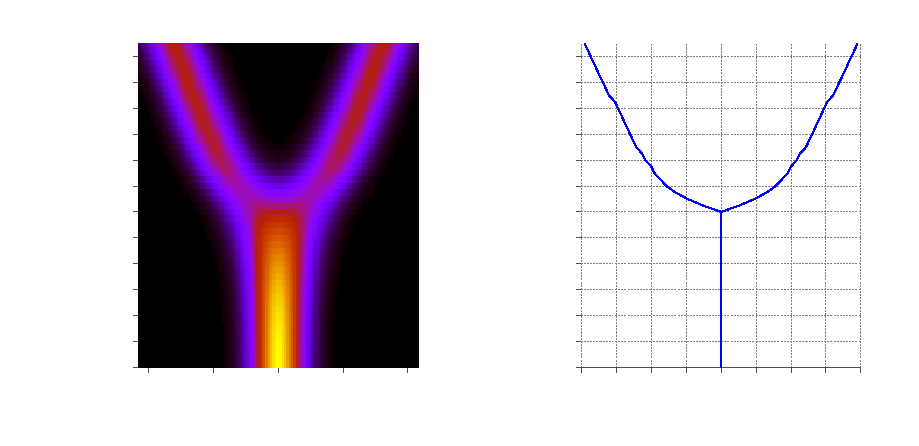
\includegraphics{images/uirCoupl}}%
    \gplfronttext
  \end{picture}%
\endgroup

  \caption{Projection into phonon coordinates (left panel) and calculated cluster distortion $d$ (right panel) for different $\lambda_{ir}$ coupling values with $u_R=0$.}
  \label{fig:uirCoupl}
\end{figure}

In the right panel of figure \ref{fig:uirCoupl} we show the cluster distortion $d$ assuming the system is found in a maximum value of the projection into phonon coordinates.
Here we can see that the observed cluster distortion of $\sim 0.13$ \AA\ \cite{MustredeLeon1990} is reproduced in the intermedite coupling values. 
In particular, $\lambda_{ir}=0.1263$ eV reproduces that distortion.

Figure \ref{fig:phononProjGrdPol} shows the ground and first excitted states projected into phonon coordinates $(u_R,u_{ir})$ for $\lambda_{ir}$ values in the three regimes.
The projection along $u_R$, as previously stated, is a simple gaussian in all cases.
In the middle coupling regime, with $\lambda_{ir}=0.1263$ eV, there are clearly two peaks present although they are not fully separated.
Since the probability amplitude is not neglible between the two maxima the system can \textit{tunnel} between both possible configurations with the longer distance in the first oxygen or the second bond.
This observation can be interpreted as a dynamic distortion in the cluster that can only be experimentally identifyied with a technique with a similar timescale (see discussion in secion \ref{sec:dynamic_dist}). 
For greater coupling values the two peaks are completely separated and the distortion becomes static.

\begin{figure}[ht]
  \centering
  \input{images/phononProjGrdPol}
  \caption[Ground and first excited states projected into phonon coordinates.]
  {Projection into phonon coordinates for the ground (top) and first excited (bottom) states for three different values of the coupling parameter $\lambda_{ir}$.}
  \label{fig:phononProjGrdPol}
\end{figure}

% Figure of projection into definite electron-occupation basis for both, the ground and polaron-tunneling state

The polaron-tunneling energy $\hbar\omega_T$, at the relevant $\lambda_{ir}=0.1263$ eV is 141.39 cm$^{-1}$.

\section{Bipolaron binding energy}
\label{sec:grd-binding-energy}

The energy of the ground state changes with the coupling parameter $\lambda_{ir}$.
The change in energy, $\Delta\omega_{g}$, between the coupled and uncoupled systems can be identified as the \textit{formation energy}.
In particular, in the region where there is bipolaronic objects present, $\Delta\omega_{g}$ can be interpreted as the \textit{bipolaron binding energy}. 
In figure \ref{fig:polaronFormation} we show the dependency of $\Delta\omega_{g}$ with $\lambda_{ir}$, where we defined

\begin{equation}
  \label{eq:pol-energy}
  \Delta\omega_{g}(\lambda_{ir}) = \omega_{g}(\lambda_{ir} = 0) - \omega_{g}(\lambda_{ir})
\end{equation}

\begin{figure}[ht]
  \centering
  \input{images/polaronFormation}
  \caption{Bipolaron formation energy as a function of the $\lambda_{ir}$ coupling. The vertical line is drawn at the relevant value $\lambda_{ir}=0.1263$ eV.}
  \label{fig:polaronFormation}
\end{figure}

We observe a monotonical behaviour with small dependency in the weak coupling regime becoming stronger with greater coupling values.
In particular, for the $\lambda_{ir}=0.1263$ eV value, which reproduces the observed distortion, we find $\Delta\omega_{g}(0.1263$ eV$) = \sim 38$ meV.
This value compares favorably with the value obtained from femtosecond time-domain spectroscopy ($\sim 45$ meV) for YBa$_2$Cu$_3$O$_7$ \cite{Demsar1999}. 
We also find that if we consider a smaller electron-lattice coupling such that the distortion is 0.08 \AA, as that observed for in plane Cu(2)-O in La$_{1.85}$Sr$_{0.15}$CuO$_4$ \cite{Bianconi1996}, we obtain $E_p \sim 35$ meV, which is also comparable to estimates for the pseudogap formation energy in this system (see Fig. 4b in \cite{Kusar2005}).

\section{Isotopic effects in bipolaron formation}
\label{sec:grd-isotopic}

We turn our attention now to the isotopic shift, $\Delta_g$, of $\omega_g$ under the $^{16}$O$\rightarrow ^{18}$O substitution as defined in (\ref{eq:isot-shift-def-grd}).
Figure \ref{fig:isotPolaronFormation} shows $\Delta_g$ as a function of $\lambda_{ir}$.
Contrary to other isotopic shifts, it does not change sign.
However it shows a maximum in the middle coupling regime, reminiscent of the maximums, minimums and inflection points in the isotopic shifts of all other excitations.

\begin{figure}[ht]
  \centering
  % GNUPLOT: LaTeX picture with Postscript
\begingroup
  \makeatletter
  \providecommand\color[2][]{%
    \GenericError{(gnuplot) \space\space\space\@spaces}{%
      Package color not loaded in conjunction with
      terminal option `colourtext'%
    }{See the gnuplot documentation for explanation.%
    }{Either use 'blacktext' in gnuplot or load the package
      color.sty in LaTeX.}%
    \renewcommand\color[2][]{}%
  }%
  \providecommand\includegraphics[2][]{%
    \GenericError{(gnuplot) \space\space\space\@spaces}{%
      Package graphicx or graphics not loaded%
    }{See the gnuplot documentation for explanation.%
    }{The gnuplot epslatex terminal needs graphicx.sty or graphics.sty.}%
    \renewcommand\includegraphics[2][]{}%
  }%
  \providecommand\rotatebox[2]{#2}%
  \@ifundefined{ifGPcolor}{%
    \newif\ifGPcolor
    \GPcolortrue
  }{}%
  \@ifundefined{ifGPblacktext}{%
    \newif\ifGPblacktext
    \GPblacktextfalse
  }{}%
  % define a \g@addto@macro without @ in the name:
  \let\gplgaddtomacro\g@addto@macro
  % define empty templates for all commands taking text:
  \gdef\gplbacktext{}%
  \gdef\gplfronttext{}%
  \makeatother
  \ifGPblacktext
    % no textcolor at all
    \def\colorrgb#1{}%
    \def\colorgray#1{}%
  \else
    % gray or color?
    \ifGPcolor
      \def\colorrgb#1{\color[rgb]{#1}}%
      \def\colorgray#1{\color[gray]{#1}}%
      \expandafter\def\csname LTw\endcsname{\color{white}}%
      \expandafter\def\csname LTb\endcsname{\color{black}}%
      \expandafter\def\csname LTa\endcsname{\color{black}}%
      \expandafter\def\csname LT0\endcsname{\color[rgb]{1,0,0}}%
      \expandafter\def\csname LT1\endcsname{\color[rgb]{0,1,0}}%
      \expandafter\def\csname LT2\endcsname{\color[rgb]{0,0,1}}%
      \expandafter\def\csname LT3\endcsname{\color[rgb]{1,0,1}}%
      \expandafter\def\csname LT4\endcsname{\color[rgb]{0,1,1}}%
      \expandafter\def\csname LT5\endcsname{\color[rgb]{1,1,0}}%
      \expandafter\def\csname LT6\endcsname{\color[rgb]{0,0,0}}%
      \expandafter\def\csname LT7\endcsname{\color[rgb]{1,0.3,0}}%
      \expandafter\def\csname LT8\endcsname{\color[rgb]{0.5,0.5,0.5}}%
    \else
      % gray
      \def\colorrgb#1{\color{black}}%
      \def\colorgray#1{\color[gray]{#1}}%
      \expandafter\def\csname LTw\endcsname{\color{white}}%
      \expandafter\def\csname LTb\endcsname{\color{black}}%
      \expandafter\def\csname LTa\endcsname{\color{black}}%
      \expandafter\def\csname LT0\endcsname{\color{black}}%
      \expandafter\def\csname LT1\endcsname{\color{black}}%
      \expandafter\def\csname LT2\endcsname{\color{black}}%
      \expandafter\def\csname LT3\endcsname{\color{black}}%
      \expandafter\def\csname LT4\endcsname{\color{black}}%
      \expandafter\def\csname LT5\endcsname{\color{black}}%
      \expandafter\def\csname LT6\endcsname{\color{black}}%
      \expandafter\def\csname LT7\endcsname{\color{black}}%
      \expandafter\def\csname LT8\endcsname{\color{black}}%
    \fi
  \fi
  \setlength{\unitlength}{0.0500bp}%
  \begin{picture}(6802.00,3968.00)%
    \gplgaddtomacro\gplbacktext{%
      \colorrgb{0.31,0.31,0.31}%
      \put(814,751){\makebox(0,0)[r]{\strut{} 5}}%
      \colorrgb{0.31,0.31,0.31}%
      \put(814,1243){\makebox(0,0)[r]{\strut{} 6}}%
      \colorrgb{0.31,0.31,0.31}%
      \put(814,1735){\makebox(0,0)[r]{\strut{} 7}}%
      \colorrgb{0.31,0.31,0.31}%
      \put(814,2227){\makebox(0,0)[r]{\strut{} 8}}%
      \colorrgb{0.31,0.31,0.31}%
      \put(814,2719){\makebox(0,0)[r]{\strut{} 9}}%
      \colorrgb{0.31,0.31,0.31}%
      \put(814,3211){\makebox(0,0)[r]{\strut{} 10}}%
      \colorrgb{0.31,0.31,0.31}%
      \put(814,3703){\makebox(0,0)[r]{\strut{} 11}}%
      \colorrgb{0.31,0.31,0.31}%
      \put(993,484){\makebox(0,0){\strut{} 0}}%
      \colorrgb{0.31,0.31,0.31}%
      \put(2075,484){\makebox(0,0){\strut{} 0.05}}%
      \colorrgb{0.31,0.31,0.31}%
      \put(3158,484){\makebox(0,0){\strut{} 0.1}}%
      \colorrgb{0.31,0.31,0.31}%
      \put(4240,484){\makebox(0,0){\strut{} 0.15}}%
      \colorrgb{0.31,0.31,0.31}%
      \put(5323,484){\makebox(0,0){\strut{} 0.2}}%
      \colorrgb{0.31,0.31,0.31}%
      \put(6405,484){\makebox(0,0){\strut{} 0.25}}%
      \csname LTb\endcsname%
      \put(176,2227){\rotatebox{-270}{\makebox(0,0){\strut{}$\Delta_g (meV)$}}}%
      \put(3699,154){\makebox(0,0){\strut{}$\lambda_{ir}$ (eV)}}%
      \put(3807,1105){\makebox(0,0)[l]{\strut{}\scriptsize$\lambda_{ir}=0.1263$}}%
    }%
    \gplgaddtomacro\gplfronttext{%
    }%
    \gplbacktext
    \put(0,0){\includegraphics{images/isotPolaronFormation}}%
    \gplfronttext
  \end{picture}%
\endgroup

  \caption{Isotopic shift of the bipolaron formation energy. The vertical line is placed at the relevant value $\lambda_{ir}=0.1263$.}
  \label{fig:isotPolaronFormation}
\end{figure}




\chapter{States with more than one infrared phonons}
\label{chap:more_ir}

Section about the states with 2 and 3 infrared phonons and their particular behaviour.

\section{Energy renormalization}

At large $\lambda_{ir}$ we recover the harmonic behaviour. This is analog to have a spring with a displaced equilibrium position.

\section{Projection into phonon coordinates}

State with two infrared phonons:

\begin{figure}[ht!]
\centering
\includegraphics[width=0.8\textwidth]{images/ph-second_infrared.png}
\caption{Projection into phonon coordinates of the state with 2 infrared phonons.}
\label{fig:ph-second_infrared}
\end{figure}

State with three infrared phonons:

\begin{figure}[ht!]
\centering
\includegraphics[width=0.8\textwidth]{images/ph-third_infrared.png}
\caption{Projection into phonon coordinates of the state with 3 infrared phonons.}
\label{fig:ph-third_infrared}
\end{figure}

\section{Isotopic shifts}

The isotopic shifts are different:

\begin{figure}[ht!]
\centering
\includegraphics[width=0.8\textwidth]{images/isot-2_3ir.jpg}
\caption{Isotopic shifts}
\label{fig:isot-2_3ir}
\end{figure}

\chapter{Electronic excitations}
\label{chap:electronic}

We call \textit{electronic} excitations those that, at $\lambda_{ir}=0$, arise from $H_{el}$ in (\ref{eq:full-hamiltonian}). This part of the hamiltonian

\begin{equation}\label{eq:Hel} H_{el} = \sum_n \epsilon_n \rho_n + \sum_{ \langle nm \rangle \sigma } t (c_{n \sigma }^\dagger c_{m \sigma } + H.c.) + U\sum_n \rho_{n\downarrow}\rho_{n\uparrow} \end{equation}

can be represented  as a 9x9 matrix:

\begin{equation}\label{eq:Hel-matrix} \left( \begin{array}{ccccccccc} 
U+2\epsilon &\;\;t\;\;&\;\;0\;\;&\;\;t\;\;&0&\;\;0\;\;&\;\;0\;\;&\;\;0\;\;&0 \\
t&0&t&0&t&0&0&0&0 \\
0&t&2\epsilon &0&0&t&0&0&0 \\
t&0&0&0&t&0&t&0&0 \\
0&t&0&t&U-2\epsilon &t&0&t&0 \\
0&0&t&0&t&0&0&0&t \\
0&0&0&t&0&0&2\epsilon &t&0 \\
0&0&0&0&t&0&t&0&t \\
0&0&0&0&0&t&0&t&U+2\epsilon  \end{array} \right)\end{equation}

and easily diagonalized to see that its first excited state has an energy of ~1376 cm$^{-1}$ above the  ground state.

\begin{figure}
  \centering
  \input{images/electrSpectra}
  \caption[Energy of the electronic excitations as function of $\lambda_{ir}$.]
  {Energy of the electronic excitations as function of $\lambda_{ir}$. 
    The red line corresponds to an electronic excitation with zero phonons, the blue line with one infrared phonon and the green line with one Raman phonon.
    The vertical line is placed at the relevant value $\lambda_{ir}=0.1263$ eV.}
  \label{fig:electrSpectra}
\end{figure}

\section{Projection into definite electronic occupation states}

Since we are using basis states with definite electron occupancy, from the eigenvectors of the (\ref{eq:Hel-matrix}) matrix we can directly see the projections into definite electronic occupation states. The following table summarizes those values omitting equivalent basis states:

\noindent\begin{tabular}{| c | c | c | c | c | c | c | c | c | c |}
\hline
Energy (cm$^{-1}$) & 0.0 & 1376.42 & 3825.49 & 4325.12 & 14897.84 & 15329.82 & 53933.30 & 69272.75 & 69309.3 \\
\hline
$\uparrow \downarrow \ - \ -$ & 0.00276 & 0.00000 & 0.00382 & 0.00000 & 0.00090 & 0.00000 & 0.00179 & 0.49618 & 0.49455 \\
$\uparrow\  \downarrow \ -$ & 0.20130 & 0.19717 & 0.24809 & 0.25000 & 0.04045 & 0.05283 & 0.00606 & 0.00191 & 0.00219 \\
$\uparrow \ - \ \downarrow$ & 0.08522 & 0.10566 & 0.00000 & 0.00000 & 0.41451 & 0.39434 & 0.00023 & 0.00000 & 0.00000 \\
$ - \ \uparrow \downarrow \ -$ & 0.01884 & 0.00000 & 0.00000 & 0.00000 & 0.00736 & 0.00000 & 0.97174 & 0.00000 & 0.00205 \\
\hline
\end{tabular}

We noticed\cite{GarciaSaraviaOrtizdeMontellano2013} that, for the first \textit{electronic} excitation, the projection into states with an electron in each oxygen decreases with an increasing $\lambda_{ir}$ suggesting partial charge localization.

\section{Projection into phonon coordinates}

\begin{figure}[ht!]
\centering
\includegraphics[width=0.8\textwidth]{images/ph-electronic.png}
\caption{Electronic state projected into phonon coordinates for three representative electron-lattice coupling ($\lambda_{ir}$) values.}
\label{fig:ph-electronic.png}
\end{figure}

\section{Isotopic shift}

\begin{figure}[ht!]
\centering
\includegraphics[width=0.8\textwidth]{images/isot-el.jpg}
\caption{Isotopic shift for the electronic state.}
\label{fig:isot-el}
\end{figure}


\chapter{Discussion and conclusions}
\label{chap:conclusions}

In this thesis we reviewed the evidence for the appearance of a dynamically inhomogeneous ground state in the pseudogap region. 
In this state there are bipolaronic objects which form at a characteristic temperature $T^*$. 
The manifestations of these objects in the lattice appear as dynamical local lattice distortions in regions in which the charge and lattice motion become correlated. 
The excitations of these bipolaronic objects exhibit different isotopic shifts depending on the nature of the excitation ranging from large negative to quasi-harmonic shifts. 
These peculiar shifts are consistent with experimental observations and might explain discrepancies in values determined by different techniques, as they probe different excitations depending on the time and spatial resolution of the specific technique. 
However, the role in the pairing of free fermions of these bipolaronic excitations, and enhancement of $T_c$ is not yet known. 
In this spirit, some models have considered the interaction between fermionic \textit{pairs} and bipolaronic bosonic objects \cite{Bussmann-Holder2005,Mihailovic2001,Bar-Yam1991,Bianconi2000} explaining several properties of the normal state in this pseudogap region. 

\section{Validity of the Born-Oppenheimer approximation}

It is interesting to note that, although the isotopic shifts of the ground state and lowest excitations can be either positive or negative, they all exhibit the strongest variations in the intermediate coupling regime where the eigenstates in the system are mixed and it is not possible to separate them into an \textit{electronic} and a \textit{lattice} part.
It is in this intermediate regime, where the charge and lattice movements are intrinsically correlated, that the Born-Oppenheimer approximation ceases to be valid.
An exact treatment, such as the one used in this work, is free from such an approximation, however it is computationally expensive and  only relatively small systems can feasibly be explored at the moment.

The importance of the intermediate coupling regime suggests a characteristic dynamical scale for the polaronic features in the cuprate superconductors. 
Other transition metals oxides as manganites and nickelates exhibit similar local lattice distortions however, the size of the distortion is larger in manganites ($\sim 0.2$ \AA) \cite{Tyson1996} and smaller in nickelates ($\sim 0.05$ \AA) \cite{Acosta-Alejandro2008} resulting also in different time scales. 
It is enticing to relate the particular dynamical time scale of the local lattice distortions with the presence of high-temperature superconductivity in cuprates but not in other transition metal oxides thus highlighting the relevance of model hamiltonians not relying on the adiabatic and anti-adiabatic approximations.

\section{Multicomponent superconductivity}
\label{sec:multiSuperc}

Finally, we would like to discuss the possible relevance of the bipolaronic behavior, derived from the simple Peierls-Hubbard Hamiltonian model (\ref{eq:full-hamiltonian}) to high temperature superconductivity. 
The observation of a Fermi surface in photoemission experiments \cite{Ding1996,Hussey2003} implies that, in addition to the bipolaronic objects (of bosonic character), there are also quasi-free fermions. 
As a function of doping the ratio of these two kinds of objects varies, yielding different characterizations of the ground state starting as an antiferromagnetic Mott insulator at zero doping, an inhomogeneous pseudogap phase where at least two different type of carriers coexist and ending in a Fermi-liquid metal in the overdoped region of the phase diagram. 
The fact that the highest $T_c$  is realized in this pseudogap region suggests the importance of the bipolaron bosonic objects. 
However, their role in the pairing of free fermions and enhancement of $T_c$ is not yet known. 
In order to understand this role, a natural extension of the model treated here is to couple the Halmiltonian  (\ref{eq:full-hamiltonian}) to an independent a free fermion system $H_A$ and find the corresponding excitations allowing exchange of the fermions involved in the bipolaronic objects with those in the free fermion part. 
In the spirit of the exact treatment of the bipolaronic subsystem, the simplest interaction between mobile fermions and charges forming part of a bipolaron is a linear hopping term. 
Such a term would allow the transfer of a single fermion from the mobile fermion to the bipolaron subsystems. 
In principle, in an exact treatment like this, the possibility of pair hopping would be implicitly included. 
That is not the case in a perturbative treatment, in which the single particle exchange (hopping) can be folded into the pair exchange (see \cite{Bar-Yam1991}).
If we consider the simplest free fermion system consisting only on two non interacting fermions in real space, with creation and anihilation operators $a^\dagger$ and $a$ respectively, the coupling of (\ref{eq:full-hamiltonian}) to this sytem ($H_A$) can be written as

\begin{equation}
  \label{eq:multicomponent}
  H_A = 
  E_A \sum_{\sigma, k=1,2} m_{\sigma, k} + 
  t_A \sum_{\sigma} (a_{\sigma, 1}^\dagger a_{\sigma, 2} + a_{\sigma,2}^\dagger a_{\sigma, 1}) + 
  \lambda_A \sum_{i,k,\sigma} \left( c_{i,\sigma}^\dagger a_{k,\sigma} + a_{k,\sigma}^\dagger c_{i,\sigma} \right) 
\end{equation}
% 
with $i=1,2,3$ labeling the sites in the CuO$_2$ cluster and $k=1,2$ the two sites for the free fermions. 
Here $m_{\sigma, k} = a_{\sigma, k}^\dagger a_{\sigma, k}$ is the number operator in the free fermion subsystem, $E_A$ its site energy and $\lambda_A$ parametrizes its interaction with the CuO$_2$ cluster.
This approach still allows us to use an exact treatment, albeit missing the possible extended nature of the free fermion states. 
If a perturbative approach was used instead it could be possible to replace the free fermion subsystem by a full band in $k$-space. 
In addition, an onsite Coulomb repulsion term could be added to the free electron subsystem and still feasibly perform an exact diagonalization. 
In this case the basis set, considering the same number of phonons, is two orders of magnitude larger than the one used for the original Peirles-Hubbard Hamiltonian (\ref{eq:full-hamiltonian}) but still within reach of modern computational resources.
 
In this model an increased projection of a given excitation on a double occupancy basis state of the free fermion part would be a signature of pairing mediated by the bipolaronic objects in the CuO$_2$ cluster. 
Additionally, the role played by the antiferromagnetic background present at zero doping and its interaction with both the fermionic carriers and polaronic objects has to be addressed.


\appendix
%\include{filename}

\bibliography{biblio} 						%nombre del archivo con la bibliografa
\bibliographystyle{unsrt}				%estilo de la bibliografa (unsrt = por orden de citacin)


\end{document}
